%%%%%%%%%%%%%%%%%%%%%%%%%%%%%%%%%%%%%%%%%
% Documentation report
%
% Original LaTeX-template by Huib Aldewereld
% The LaTeX-template is licensed under Creative Commons Attribution-ShareAlike 4.0 International (CC BY-SA 4.0) license
%
% Important note:
% Chapter heading images should have a 2:1 width:height ratio,
% e.g. 920px width and 460px height.
%
%%%%%%%%%%%%%%%%%%%%%%%%%%%%%%%%%%%%%%%%%

%----------------------------------------------------------------------------------------
%	PACKAGES AND OTHER DOCUMENT CONFIGURATIONS
%----------------------------------------------------------------------------------------

\documentclass[11pt,fleqn]{book} % Default font size and left-justified equations

\usepackage[top=3cm,bottom=3cm,left=1.0cm,right=1.0cm,headsep=10pt,a4paper,margin=3cm,marginparwidth=2.5cm]{geometry} % Page margins


% orginele reader gebruikte HAN-huisstijl. Op verzoek van de HAN-communicatie-afdeling aangepast
\usepackage[table, x11names]{xcolor} % Required for specifying colors by name
\definecolor{hanblack}{RGB}{0, 0, 0} % 
\definecolor{notHANred}{RGB}{0, 102, 0 } %iets wat niet de HAN-rood is.
%\definecolor{hanred}{RGB}{229, 0, 86 } %officiele rood van de HAN
\definecolor{hanwhite}{RGB}{255, 255, 255 } %officiele rood van de HAN
\definecolor{handarkgrey}{RGB}{69, 69, 69 } %officiele donker grijs van de HAN
\definecolor{hangrey}{RGB} {145, 145, 145 } %officiele grijs van de HAN
\definecolor{hanlightgrey}{RGB}{227, 227, 227 } %officiele grijs van de HAN

% Added by Jorn:
% some packages may not be needed anymore...
\usepackage{eurosym} %required voor euro (money) symbol
\usepackage{subcaption} %required for multiple images in one image.
\usepackage[T1]{fontenc} % om een letter net iets lager te plaatsen.
\interfootnotelinepenalty=10000 %footnotes niet over meerdere pagina's.
\usepackage[export]{adjustbox} %for aligning images
\usepackage{lipsum} %voor lipsum text
\usepgflibrary{arrows} % for pgf-umlsd
\usepackage{changepage} % om minipages groter the maken dan textwidth


% Margin captions (voor plaatjes / figures/ figuren/ figuur)
\usepackage{floatrow}
\floatsetup{margins=hangleft,capposition=beside,capbesideposition={top,left},floatwidth=\textwidth}
\usepackage[labelfont=bf,labelsep=newline,justification=raggedright, font=scriptsize]{caption}

% Continuous footnotes
\usepackage{chngcntr}
\counterwithout{footnote}{chapter}

% Font Settings
\usepackage{avant} % Use the Avantgarde font for headings

\usepackage{microtype} % Slightly tweak font spacing for aesthetics
\usepackage[T1]{fontenc} % Use 8-bit encoding that has 256 glyphs

% Code formats
\usepackage{Layout_files/python}
\usepackage{Layout_files/C++}
\usepackage{Layout_files/Dos}
\usepackage{Layout_files/xml}

\renewcommand{\lstlistingname}{Codevoorbeeld}
\renewcommand{\lstlistlistingname}{List of \lstlistingname s}


\usepackage[hidelinks]{hyperref}
\usepackage{array}
\usepackage{multicol}
% define centering minipage column type
\newcolumntype{P}[1]{>{\centering\arraybackslash}p{#1}}
% rotate for column headers
\usepackage{adjustbox}
\newcolumntype{R}[2]{%
    >{\adjustbox{angle=#1,lap=\width-(#2)}\bgroup}%
    l%
    <{\egroup}%
}
\newcommand*\rot{\multicolumn{1}{R{60}{1em}}}% no optional argument here, please!
\usepackage{physics,enumitem}


\usepackage[colorinlistoftodos,textsize=scriptsize]{todonotes}
\newcommand{\note}[1]{\todo[color=notHANred!60]{#1}}

\usepackage[title,titletoc]{appendix}
\renewcommand{\appendixtocname}{Appendices}

% add for bibliography:
% Bibliographybackref=true,abbreviate=false,
%\usepackage{csquotes}
%\usepackage[style=authoryear,citestyle=apa,natbib=true,autopunct=true%,backend=biber]{biblatex}
%\addbibresource{bibliography.bib} % BibTeX bibliography file
%\defbibheading{bibempty}{}

%----------------------------------------------------------------------------------------
%	VARIOUS REQUIRED PACKAGES
%----------------------------------------------------------------------------------------

\usepackage{titlesec} % Allows customization of titles

\usepackage{graphicx} % Required for including pictures
\graphicspath{{Pictures/}} % Specifies the directory where pictures are stored

\usepackage{lipsum} % Inserts dummy text

\usepackage{tikz} % Required for drawing custom shapes

\usepackage[dutch]{babel} % English language/hyphenation

\usepackage{enumitem} % Customize lists
\setlist{nolistsep} % Reduce spacing between bullet points and numbered lists

\usepackage{booktabs} % Required for nicer horizontal rules in tables

\usepackage{eso-pic} % Required for specifying an image background in the title page

\usepackage{algpseudocode}

\usepackage{framed}

%----------------------------------------------------------------------------------------
%	MAIN TABLE OF CONTENTS
%----------------------------------------------------------------------------------------

\usepackage{titletoc} % Required for manipulating the table of contents

\contentsmargin{0cm} % Removes the default margin
% Chapter text styling
\titlecontents{chapter}[1.25cm] % Indentation
{\addvspace{15pt}\large\sffamily\bfseries} % Spacing and font options for chapters
{\color{notHANred!60}\contentslabel[\Large\thecontentslabel]{1.25cm}\color{notHANred}} % Chapter number
{}  
{\color{notHANred!60}\normalsize\sffamily\bfseries\;\titlerule*[.5pc]{.}\;\thecontentspage} % Page number
% Section text styling
\titlecontents{section}[1.25cm] % Indentation
{\addvspace{5pt}\sffamily\bfseries} % Spacing and font options for sections
{\contentslabel[\thecontentslabel]{1.25cm}} % Section number
{}
{\sffamily\hfill\color{black}\thecontentspage} % Page number
[]
% Subsection text styling
\titlecontents{subsection}[1.25cm] % Indentation
{\addvspace{1pt}\sffamily\small} % Spacing and font options for subsections
{\contentslabel[\thecontentslabel]{1.25cm}} % Subsection number
{}
{\sffamily\;\titlerule*[.5pc]{.}\;\thecontentspage} % Page number
[] 

%----------------------------------------------------------------------------------------
%	MINI TABLE OF CONTENTS IN CHAPTER HEADS
%----------------------------------------------------------------------------------------

% Section text styling
\titlecontents{lsection}[0em] % Indentation
{\footnotesize\sffamily} % Font settings
{}
{}
{}

% Subsection text styling
\titlecontents{lsubsection}[.5em] % Indentation
{\normalfont\footnotesize\sffamily} % Font settings
{}
{}
{}
 
%----------------------------------------------------------------------------------------
%	PAGE HEADERS
%----------------------------------------------------------------------------------------

\usepackage{fancyhdr} % Required for header and footer configuration

\pagestyle{fancy}

\renewcommand{\chaptermark}[1]{\markboth{\sffamily\normalsize\bfseries\chaptername\ \thechapter.\ #1}{}} % Chapter text font settings
\renewcommand{\sectionmark}[1]{\markright{\sffamily\normalsize\thesection\hspace{5pt}#1}{}} % Section text font settings
\fancyhf{} \fancyhead[LE,RO]{\sffamily\normalsize\thepage} % Font setting for the page number in the header
\fancyhead[LO]{\rightmark} % Print the nearest section name on the left side of odd pages
\fancyhead[RE]{\leftmark} % Print the current chapter name on the right side of even pages
\renewcommand{\headrulewidth}{0.5pt} % Width of the rule under the header
\addtolength{\headheight}{2.5pt} % Increase the spacing around the header slightly
\renewcommand{\footrulewidth}{0pt} % Removes the rule in the footer
\fancypagestyle{plain}{\fancyhead{}\renewcommand{\headrulewidth}{0pt}} % Style for when a plain pagestyle is specified

% Removes the header from odd empty pages at the end of chapters
\makeatletter
\renewcommand{\cleardoublepage}{
\clearpage\ifodd\c@page\else
\hbox{}
\vspace*{\fill}
\thispagestyle{empty}
\newpage
\fi}

%----------------------------------------------------------------------------------------
%	THEOREM STYLES
%----------------------------------------------------------------------------------------

\usepackage{amsmath,amsfonts,amssymb,amsthm} % For math equations, theorems, symbols, etc

\newcommand{\intoo}[2]{\mathopen{]}#1\,;#2\mathclose{[}}
\newcommand{\ud}{\mathop{\mathrm{{}d}}\mathopen{}}
\newcommand{\intff}[2]{\mathopen{[}#1\,;#2\mathclose{]}}

%%%%%%%%%%%%%%%%%%%%%%%%%%%%%%%%%%%%%%%%%%%%%%%%%%%%%%%%%%%%%%%%%%%%%%%%%%%
%%%%%%%%%%%%%%%%%%%% dedicated to boxed/framed environements %%%%%%%%%%%%%%
%%%%%%%%%%%%%%%%%%%%%%%%%%%%%%%%%%%%%%%%%%%%%%%%%%%%%%%%%%%%%%%%%%%%%%%%%%%
\newtheoremstyle{rednumbox}% % Theorem style name
{0pt}% Space above
{0pt}% Space below
{\normalfont}% % Body font
{}% Indent amount
{\small\bf\sffamily\color{notHANred}}% % Theorem head font
{\;}% Punctuation after theorem head
{0.25em}% Space after theorem head
{\small\sffamily\color{notHANred}\thmname{#1}\nobreakspace\thmnumber{\@ifnotempty{#1}{}\@upn{#2}}% Theorem text (e.g. Theorem 2.1)
\thmnote{\nobreakspace\the\thm@notefont\sffamily\bfseries\color{black}---\nobreakspace#3.\\}} % Optional theorem note
\renewcommand{\qedsymbol}{$\blacksquare$}% Optional qed square

\newtheoremstyle{blacknumex}% Theorem style name
{0pt}% Space above
{0pt}% Space below
{\normalfont}% Body font
{} % Indent amount
{\small\bf\sffamily}% Theorem head font
{\;}% Punctuation after theorem head
{0.25em}% Space after theorem head
{\small\sffamily\nobreakspace\thmname{#1}\nobreakspace\thmnumber{\@ifnotempty{#1}{}\@upn{#2}}% Theorem text (e.g. Theorem 2.1)
\thmnote{\nobreakspace\the\thm@notefont\sffamily\bfseries---\nobreakspace#3.}}% Optional theorem note

\newtheoremstyle{blacknumbox} % Theorem style name
{0pt}% Space above
{0pt}% Space below
{\normalfont}% Body font
{}% Indent amount
{\small\bf\sffamily}% Theorem head font
{\;}% Punctuation after theorem head
{0.25em}% Space after theorem head
{\small\sffamily\thmname{#1}\nobreakspace\thmnumber{\@ifnotempty{#1}{}\@upn{#2}}% Theorem text (e.g. Theorem 2.1)
\thmnote{\nobreakspace\the\thm@notefont\sffamily\bfseries---\nobreakspace#3.}}% Optional theorem note

%%%%%%%%%%%%%%%%%%%%%%%%%%%%%%%%%%%%%%%%%%%%%%%%%%%%%%%%%%%%%%%%%%%%%%%%%%%
%%%%%%%%%%%%% dedicated to non-boxed/non-framed environments %%%%%%%%%%%%%
%%%%%%%%%%%%%%%%%%%%%%%%%%%%%%%%%%%%%%%%%%%%%%%%%%%%%%%%%%%%%%%%%%%%%%%%%%%
\newtheoremstyle{rednum}% % Theorem style name
{5pt}% Space above
{5pt}% Space below
{\normalfont}% % Body font
{}% Indent amount
{\small\bf\sffamily\color{notHANred}}% % Theorem head font
{\;}% Punctuation after theorem head
{0.25em}% Space after theorem head
{\small\sffamily\color{notHANred}\thmname{#1}\nobreakspace\thmnumber{\@ifnotempty{#1}{}\@upn{#2}}% Theorem text (e.g. Theorem 2.1)
\thmnote{\nobreakspace\the\thm@notefont\sffamily\bfseries\color{black}---\nobreakspace#3.}} % Optional theorem note
\renewcommand{\qedsymbol}{$\blacksquare$}% Optional qed square
\makeatother

% Defines the theorem text style for each type of theorem to one of the three styles above
\newcounter{dummy} 
\numberwithin{dummy}{section}

\theoremstyle{rednumbox}
\newtheorem{theoremeT}[dummy]{Stelling}
\newtheorem{notationT}[dummy]{Notatie}
\newtheorem{problem}{Probleem}[chapter]
\newtheorem{exerciseT}{Opgave}[chapter]
\newtheorem{answerT}{Uitwerking}[section]
\newtheorem{definitionT}{Definitie}[chapter]


\theoremstyle{blacknumex}
\newtheorem{exampleT}{Voorbeeld}[chapter]

\theoremstyle{blacknumbox}
\newtheorem{vocabularyT}{Vocabulair}[chapter]
\newtheorem{asideT}{Terzijde}[chapter]
\newtheorem{algorithmT}{Algoritme}[chapter]
\newtheorem{corollaryT}[dummy]{Corrolarium}

\theoremstyle{rednum}
\newtheorem{proposition}[dummy]{Propositie}
\newtheorem{axiom}{Axioma}[chapter]

%----------------------------------------------------------------------------------------
%	DEFINITION OF COLORED BOXES
%----------------------------------------------------------------------------------------

\RequirePackage[framemethod=default]{mdframed} % Required for creating the theorem, definition, exercise and corollary boxes

% Theorem box
\newmdenv[skipabove=7pt,
skipbelow=7pt,
backgroundcolor=hanblack!10,
linecolor=hanblack,
innerleftmargin=5pt,
innerrightmargin=5pt,
innertopmargin=5pt,
leftmargin=0cm,
rightmargin=0cm,
innerbottommargin=5pt]{tBox}

% Exercise box	 
\newmdenv[skipabove=7pt,
skipbelow=7pt,
rightline=false,
leftline=true,
topline=false,
bottomline=false,
backgroundcolor=hanblack!10,
linecolor=notHANred,
innerleftmargin=5pt,
innerrightmargin=5pt,
innertopmargin=5pt,
innerbottommargin=5pt,
leftmargin=0cm,
rightmargin=0cm,
linewidth=4pt]{eBox}	

% Definition box
\newmdenv[skipabove=7pt,
skipbelow=7pt,
rightline=false,
leftline=true,
topline=false,
bottomline=false,
linecolor=hanblack,
innerleftmargin=5pt,
innerrightmargin=5pt,
innertopmargin=0pt,
leftmargin=0cm,
rightmargin=0cm,
linewidth=4pt,
innerbottommargin=0pt]{dBox}

% Corollary box
\newmdenv[skipabove=7pt,
skipbelow=7pt,
rightline=false,
leftline=true,
topline=false,
bottomline=false,
linecolor=notHANred,
backgroundcolor=hanlightgrey,
innerleftmargin=5pt,
innerrightmargin=5pt,
innertopmargin=5pt,
leftmargin=0cm,
rightmargin=0cm,
linewidth=4pt,
innerbottommargin=5pt]{cBox}

% Example box
\newmdenv[skipabove=7pt,
skipbelow=7pt,
rightline=false,
leftline=true,
topline=false,
bottomline=false,
linecolor=notHANred,
backgroundcolor=hanlightgrey,
innerleftmargin=5pt,
innerrightmargin=5pt,
innertopmargin=5pt,
leftmargin=0cm,
rightmargin=0cm,
linewidth=4pt,
innerbottommargin=0pt]{exBox}

% Creates an environment for each type of theorem and assigns it a theorem text style from the "Theorem Styles" section above and a coloured box from above
\newenvironment{theorem}{\begin{tBox}\begin{theoremeT}}{\end{theoremeT}\end{tBox}}
\newenvironment{notation}{\begin{tBox}\begin{notationT}}{\end{notationT}\end{tBox}}
\newenvironment{exercise}{\begin{eBox}\begin{exerciseT}}{\end{exerciseT}\end{eBox}}	
\newenvironment{answer}{\begin{eBox}\begin{answerT}}{\end{answerT}\end{eBox}}
\newenvironment{definition}{\begin{dBox}\begin{definitionT}}{\end{definitionT}\end{dBox}}	
\newenvironment{example}{\begin{exBox}\begin{exampleT}}{\end{exampleT}\end{exBox}}
%\newenvironment{example}{\begin{exampleT}}{\hfill{\tiny\ensuremath{\blacksquare}}\end{exampleT}}	
\newenvironment{algorithm}{\begin{dBox}\begin{algorithmT}}{\hfill{\tiny\ensuremath{\blacksquare}}\end{algorithmT}\end{dBox}}	
\newenvironment{corollary}{\begin{cBox}\begin{corollaryT}}{\end{corollaryT}\end{cBox}}	
\newenvironment{vocabulary}{\begin{cBox}\begin{vocabularyT}}{\end{vocabularyT}\end{cBox}}	
\newenvironment{aside}{\begin{cBox}\begin{asideT}}{\end{asideT}\end{cBox}}

%----------------------------------------------------------------------------------------
%	REMARK ENVIRONMENT
%----------------------------------------------------------------------------------------

\newenvironment{remark}{\par\vspace{10pt}\small % Vertical white space above the remark and smaller font size
\begin{list}{}{
\leftmargin=35pt % Indentation on the left
\rightmargin=25pt}\item\ignorespaces % Indentation on the right
\makebox[-2.5pt]{\begin{tikzpicture}[overlay]
\node[draw=notHANred!60,line width=1pt,circle,fill=notHANred!25,font=\sffamily\bfseries,inner sep=2pt,outer sep=0pt] at (-15pt,0pt){\textcolor{notHANred}{R}};\end{tikzpicture}} % Orange R in a circle
\advance\baselineskip -1pt}{\end{list}\vskip5pt} % Tighter line spacing and white space after remark

%----------------------------------------------------------------------------------------
%	SECTION NUMBERING IN THE MARGIN
%----------------------------------------------------------------------------------------

\makeatletter
\renewcommand{\@seccntformat}[1]{\llap{\textcolor{notHANred}{\csname the#1\endcsname}\hspace{1em}}}                    
\renewcommand{\section}{\@startsection{section}{1}{\z@}
{-4ex \@plus -1ex \@minus -.4ex}
{1ex \@plus.2ex }
{\normalfont\large\sffamily\bfseries}}
\renewcommand{\subsection}{\@startsection {subsection}{2}{\z@}
{-3ex \@plus -0.1ex \@minus -.4ex}
{0.5ex \@plus.2ex }
{\normalfont\sffamily\bfseries}}
\renewcommand{\subsubsection}{\@startsection {subsubsection}{3}{\z@}
{-2ex \@plus -0.1ex \@minus -.2ex}
{.2ex \@plus.2ex }
{\normalfont\small\sffamily\bfseries}}                        
\renewcommand\paragraph{\@startsection{paragraph}{4}{\z@}
{-2ex \@plus-.2ex \@minus .2ex}
{.1ex}
{\normalfont\small\sffamily\bfseries}}

%----------------------------------------------------------------------------------------
%	HYPERLINKS IN THE DOCUMENTS
%----------------------------------------------------------------------------------------

% For an unclear reason, the package should be loaded now and not later
%\usepackage{hyperref}
%\hypersetup{hidelinks,backref=true,pagebackref=true,hyperindex=true,colorlinks=false,breaklinks=true,urlcolor= notHANred,bookmarks=true,bookmarksopen=false,pdftitle={Title},pdfauthor={Author}}

%----------------------------------------------------------------------------------------
%	CHAPTER HEADINGS
%----------------------------------------------------------------------------------------

% The set-up below should be (sadly) manually adapted to the overall margin page septup controlled by the geometry package loaded in the main.tex document. It is possible to implement below the dimensions used in the goemetry package (top,bottom,left,right)... TO BE DONE

\newcommand{\thechapterimage}{}
\newcommand{\chapterimage}[1]{\renewcommand{\thechapterimage}{#1}}

% Numbered chapters with mini tableofcontents
\def\thechapter{\arabic{chapter}}
\def\@makechapterhead#1{
\thispagestyle{empty}
{\centering \normalfont\sffamily
\ifnum \c@secnumdepth >\m@ne
\if@mainmatter
\startcontents
\begin{tikzpicture}[remember picture,overlay]
\node at (current page.north west)
{\begin{tikzpicture}[remember picture,overlay]
\node[anchor=north west,inner sep=0pt] at (0,0) {\includegraphics[width=\paperwidth]{\thechapterimage}};
%%%%%%%%%%%%%%%%%%%%%%%%%%%%%%%%%%%%%%%%%%%%%%%%%%%%%%%%%%%%%%%%%%%%%%%%%%%%%%%%%%%%%
% Commenting the 3 lines below removes the small contents box in the chapter heading
%\fill[color=hanblack!10!white,opacity=.6] (1cm,0) rectangle (8cm,-7cm);
%\node[anchor=north west] at (1.1cm,.35cm) {\parbox[t][8cm][t]{6.5cm}{\huge\bfseries\flushleft \printcontents{l}{1}{\setcounter{tocdepth}{2}}}};
\draw[anchor=west] (5cm,-8.5cm) node [fill=hanblack,text opacity=1,draw=hanblack,draw opacity=1,line width=1.5pt,fill opacity=1,inner sep=12pt]{\huge\sffamily\bfseries\textcolor{hanwhite}{\thechapter. #1 \strut\makebox[22cm]{}}};
%%%%%%%%%%%%%%%%%%%%%%%%%%%%%%%%%%%%%%%%%%%%%%%%%%%%%%%%%%%%%%%%%%%%%%%%%%%%%%%%%%%%%
\end{tikzpicture}};
\end{tikzpicture}}
\par\vspace*{230\p@}
\fi
\fi}

% Unnumbered chapters without mini tableofcontents (could be added though) 
%hier staat de stijl van de inhoudsopgave:
\def\@makeschapterhead#1{
\thispagestyle{empty}
{\centering \normalfont\sffamily
\ifnum \c@secnumdepth >\m@ne
\if@mainmatter
\begin{tikzpicture}[remember picture,overlay]
\node at (current page.north west)
{\begin{tikzpicture}[remember picture,overlay]
\node[anchor=north west,inner sep=0pt] at (0,0) {\includegraphics[width=\paperwidth]{\thechapterimage}};
\draw[anchor=west] (5cm,-8.5cm) node [fill=hanblack,fill opacity=1.0,inner sep=12pt,text opacity=1,draw=hanblack,draw opacity=1,line width=1.5pt]{\huge\sffamily\bfseries\textcolor{hanwhite}{#1 \strut\makebox[22cm]{}}};
\end{tikzpicture}};
\end{tikzpicture}}
\par\vspace*{230\p@}
\fi
\fi
}
\makeatother

\makeatletter
\def\unfootnote{\xdef\@thefnmark{}\@footnotetext}
\makeatother % Insert the commands.tex file which contains the majority of the structure behind the template

\tikzstyle{coverbox} = [fill=black, rectangle, inner sep=7pt, inner ysep=12pt, fill opacity=1, text opacity=1]
\usetikzlibrary{arrows, shapes, positioning, arrows.meta,decorations.pathreplacing,matrix,positioning,3d, automata, positioning,fit,calc}
\tikzstyle{blArrow}=[line width=1mm,draw=black!80,-triangle 45,postaction={draw, line width=3mm, shorten >=4mm, -}]

\tikzset{xyp/.style={canvas is xy plane at z=#1}}
\tikzset{xzp/.style={canvas is xz plane at y=#1}}
\tikzset{yzp/.style={canvas is yz plane at x=#1}}

%


\begin{document}

%----------------------------------------------------------------------------------------
%	TITLE PAGE
%----------------------------------------------------------------------------------------

\begingroup
\thispagestyle{empty}
\AddToShipoutPicture*{\put(-275, -50){
		\parbox[b][\paperheight]{\paperwidth}{%
			\vfill
			\centering
			\includegraphics[height=1.1\paperheight]{Pictures/cc_pixabay_cover_robot.jpg}
			\vfill
}}} % Image background
\begin{center}
	\begin{tikzpicture} [remember picture,overlay]
	\node [coverbox] (title) at (0, -1) {
		\begin{minipage}{\textwidth}
		\centering
		\normalfont\fontsize{35}{35}\sffamily\selectfont
		\textbf{\color{hanwhite}{ROS 2}}\\ % book title
		{\LARGE \color{hanwhite}{Een uitgebreide introductie}} % sub title
		\end{minipage}
	};
	\node [coverbox] (authors) at (0, -18.5) {
		\begin{minipage}{\textwidth}
		\centering
		\normalfont\fontsize{24}{24}\sffamily\selectfont
		{\huge\color{hanwhite}{Jorn Bunk}}
		\end{minipage}
	};
	\node (logo) at (2, -25) {
		
\includegraphics[width=2cm, right]{HAN_merkteken_descriptor-144}
	};
	
	\end{tikzpicture}
\end{center}
\endgroup

%----------------------------------------------------------------------------------------
%	COPYRIGHT PAGE
%----------------------------------------------------------------------------------------

\newpage


\includegraphics[width=7cm, right]{HAN_merkteken_descriptor-144}
~\vfill
\thispagestyle{empty}

\noindent \textsc{Dit document is gemaakt voor studenten van AIM van de Hogeschool Arnhem en Nijmegen. Dit document is gelicentieerd onder een \textit{Creative Commons Attribution-ShareAlike 4.0 International (CC BY-SA 4.0)} licentie. Alle codevoorbeelden zijn gelicentieerd onder een \textit{Attribution 4.0 International (CC BY 4.0)} licentie.}\\ % License information

\noindent \url{www.han.nl}\\ % URL

\noindent Dit document is tot stand gekomen door bijdrages en feedback van:\\
\\[0.2cm]
\begin{tabular}{|p{3.5cm}|p{4cm}|p{4cm}|}
\hline
Jorn Bunk & Hogeschooldocent ESD & Auteur\\
Wilrick Bakker & Student HAN & Feedback \\
Erik Brilleman & Student HAN & Feedback\\
Sandra ter Maat & Student HAN & Feedback \\
Daan Smienk & Student HU & Feedback \\
Sua Wilhelm & Student HU & Feedback \\
Huib Aldewereld & & \LaTeX-template \\
\hline
\end{tabular}\\[1cm]

\noindent \textit{Versie 1.1, april 2022} % Printing/edition date

%----------------------------------------------------------------------------------------
%	TABLE OF CONTENTS
%----------------------------------------------------------------------------------------

\chapterimage{cc_pixabay_header_bureau} % Table of contents heading image

\pagestyle{empty} % No headers
\setcounter{tocdepth}{1}
\tableofcontents % Print the table of contents itself

%\cleardoublepage % Forces the first chapter to start on an odd page so it's on the right

\pagestyle{fancy} % Print headers again

%----------------------------------------------------------------------------------------
%	CHAPTERS
%----------------------------------------------------------------------------------------

% Chapter 1
\chapterimage{cc_pixabay_header_robot_books.png} 
\chapter{Introductie}

\noindent Met deze reader verkrijgt de lezer een stevige fundatie voor het gebruik van ROS 2 aan de hand van concrete codevoorbeelden. ROS is een open source software framework en komt met veel tools voor het programmeren, het compilen van code, het testen en het simuleren van hardware. Een belangrijke eigenschap van ROS is dat het de communicatie verzorgt tussen de verschillende processen (``robot onderdelen''). ROS maakt het hiermee mogelijk software te schrijven voor \'e\'en onderdeel zonder dat men zich zorgen hoeft te maken over elk klein detail van de andere onderdelen. De flexibiliteit en herbruikbaarheid van code en hardware wordt hiermee vergroot. Een in ROS geprogrammeerde ultra-sound sensor kan zowel werken op de Care-O-Bot 4 als op de Terminator\footnote{De aanname is dat Arnold Schwarzenegger draait met ROS (\url{https://www.imdb.com/title/tt0088247/}).}. Het is dan ook niet gek dat de meeste robot(onderdelen)fabrikanten software leveren die werkt met ROS. Hiermee kan hun hardware flexibel worden gebruikt in de meest uiteenlopende projecten. Daarnaast zorgt de open-source-community van ROS dat vele libraries beschikbaar zijn.

\begin{figure}[ht]
\begin{center}
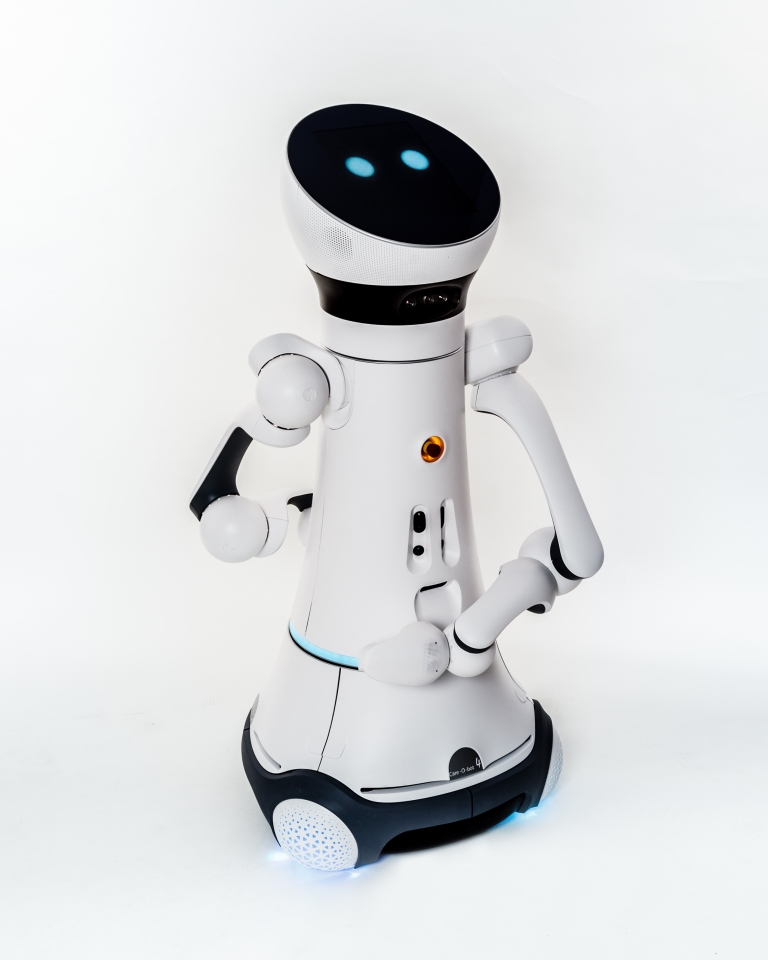
\includegraphics[scale=0.15]{Care-O-bot_4}\\
\end{center}
\caption{De zorgrobot Care-O-bot 4\\\tiny{(Foto door Fraunhofer IPA)}}\label{fig:care-o-bot4}
\end{figure}

De voordelen van ROS zijn zichtbaar bij de zorgrobot Care-O-Bot 4 (zie figuur \ref{fig:care-o-bot4}). Deze heeft verschillende sensoren (microfoon, knoppen, camera's, LiDar) en meerdere actuatoren (wielen, robotarmen, scherm, etc.) die met elkaar moeten samenwerken en communiceren. Elke sensor en actuator heeft zijn eigen (programmeer)uitdagingen die we graag, voor zo ver mogelijk, per onderdeel aanpakken. Verder willen we graag flexibel zijn in welke sensoren en actuatoren de Care-O-Bot gebruikt. ROS helpt ons hierbij. Het doel van ROS is het verzorgen van een standaard voor robot software development dat resulteert in software dat werkt op elke robot. 

De reader start bij de basis, een simpele ROS-node, en gaat vervolgens in op de drie manieren van communicatie in ROS 2. Naast de codevoorbeelden in de reader is zijn er nog meer codevoorbeelden beschikbaar op de git. Voordat men zijn/haar eigen code met ROS gaat schrijven raden wij sterk aan of hoofdstuk 2 en 3 van deze reader te lezen en de stappen van appendix \ref{chp:HelloNode_package} te doorlopen.\\

Deze reader is ontwikkeld ter ondersteuning van de cursus \textit{World} van de Hogeschool Arnhem en Nijmegen. De reader bevat de belangrijkste functionaliteiten van ROS 2, maar heeft een focus op de C++code. Meer informatie over ROS 2 kan men vinden in de documentatie van ROS 2:
\begin{center}
    \url{https://docs.ros.org/en/foxy/}
\end{center}

Voordat de lezer vol enthousiasme de reader in duikt raden wij aan om eerst ROS 2 te installeren. 

\section{Installatie en gebruik}
Voor de installatie van ROS verwijzen we naar de tutorial van ROS. De auteur heeft gebruik gemaakt van ROS 2 Foxy Fitzroy op Linux.
\begin{center}
    \url{https://docs.ros.org/en/foxy/Installation.html}
\end{center}

\noindent 

\noindent Met ROS 2 maken we gebruik van de library \textit{rclcpp}. De documentatie hiervan is te vinden op:
\begin{center}
    \url{http://docs.ros2.org/latest/api/rclcpp/}
\end{center}

\vspace{1cm}

\chapterimage{cc_pixabay_header_bee}
\chapter{Nodes}
 \label{chp:ROS_nodes}
% http://docs.ros2.org/bouncy/api/rclcpp/classrclcpp_1_1_node.html 
%afgekeken bij: https://roboticsbackend.com/write-minimal-ros2-cpp-node/
\textit{Dit hoofdstuk gaat in op C++code voor het maken van een ROS-node. De stappen voor het maken van een ROS-package en het runnen van de node uit dit hoofdstuk zijn te vinden in appendix \ref{chp:HelloNode_package}.}\\

\noindent De basis van een ROS-programma zijn de nodes. Elke node is een proces en vaak verantwoordelijke voor \'e\'en taak of onderdeel. Dit kunnen dus processen zijn die hardware aansturen, maar kunnen ook processen zijn die sensordata verwerken (bijvoorbeeld beeldherkenning), de business logic afhandelen (de ``AI'') of berekeningen doen die nodig zijn voor het aansturen van andere processen. In dit hoofdstuk bekijken wat, qua code, een node precies is en hoe we het gebruiken.

In codevoorbeeld \ref{code:min_ROSnode} zien we het maken van de meest simpele node en het starten van deze node. Deze node doet niks, maar we zien hier wel dat we de node een shared pointer moeten maken, zodat vervolgens ROS het met de commando \textit{rclcpp::spin()} er een thread van kan maken. 
\begin{lstlisting}[language=C++, caption={Het maken en runnen van een minimalistische ROS-Node.}, firstnumber=0, label={code:min_ROSnode}]
// import the ROS2 core lib:
#include "rclcpp/rclcpp.hpp" 

int main(int argc, char **argv)
{
    // start ROS2:
    rclcpp::init(argc, argv);
    // create a node with the name "my_node_name" and
    // make it a shared pointer
    auto node = std::make_shared<rclcpp::Node>("my_node_name");
    // run the node (until you kill it (ctrl-c)):
    rclcpp::spin(node);
    // stop ROS2:
    rclcpp::shutdown(); 
    return 0;
}
\end{lstlisting}

\noindent Als we onze eigen ROSnode willen definiëren dan doen we dat door een subclass te maken van de rclcpp::Node. De initialisatie van deze subclass moet natuurlijk ook in een sharedpointer, zodat we er een thread binnen ROS van kunnen maken met het commando \textit{rclcpp::spin()}. In codevoorbeeld \ref{code:min_eigen_ROSnode_hpp}, \ref{code:min_eigen_ROSnode_cpp} en \ref{code:min_eigen_ROSnode_main} zien we dit uitgewerkt. De bestanden zijn netjes gesplitst in een een header-file, source file en de main die de node opstart. Buiten bestaan en zijn superclass aanmaken doet de node van de codevoorbeelden nog niks. Let op: De constructor van de superclass rclcpp::Node heeft als parameter de naam van de node. Elke node moet een unieke naam hebben.

\begin{lstlisting}[language=C++, caption={EmptyNode.hpp}, firstnumber=0, label={code:min_eigen_ROSnode_hpp}]
#include "rclcpp/rclcpp.hpp" 

// create our own Node as a subclass of Node:
class EmptyNode : public rclcpp::Node{
public:
    // constructor is the only mandatory function: 
    EmptyNode();
};
\end{lstlisting}

\begin{lstlisting}[language=C++, caption={EmptyNode.cpp}, firstnumber=0, label={code:min_eigen_ROSnode_cpp}]
#include "rclcpp/rclcpp.hpp" 
#include "EmptyNode.hpp"

// the constructor initialized the super class Node:
EmptyNode::EmptyNode() : Node("EmptyNode"){ }
\end{lstlisting}

\begin{lstlisting}[language=C++, caption={main.cpp}, firstnumber=0, label={code:min_eigen_ROSnode_main}]
#include "rclcpp/rclcpp.hpp"
#include "EmptyNode.hpp"

int main(int argc, char **argv){
    rclcpp::init(argc, argv);
    
    // create a EmptyNode and
    // make it a shared pointer:
    auto node = std::make_shared<EmptyNode>();
    
    rclcpp::spin(node); 
    rclcpp::shutdown(); 
    return 0;
}
\end{lstlisting}

\noindent In codevoorbeelden \ref{code:hello_world_ROSnode_hpp}, \ref{code:hello_world_ROSnode_cpp} en \ref{code:hello_world_ROSnode_main} zien we een node die wel wat doet. De node HelloNode print achter elkaar ``Hello World!''. Hiervoor gebruiken we de functie \textit{timerCallback()} die ``Hello World!'' print en een timer die deze functie aanroept. De class maakt hiervoor gebruik van een ROS2 timer die we kunnen krijgen van de functie \textit{create\_wall\_timer()} van de superclass \textit{rclcpp::Node}. We ontleden de code onder de codevoorbeelden. 

\begin{lstlisting}[language=C++, caption={HelloNode.hpp}, firstnumber=0, label={code:hello_world_ROSnode_hpp}]
#include "rclcpp/rclcpp.hpp"

class HelloNode : public rclcpp::Node
{
public:
    HelloNode();

private:
    // the function to be called by the timer:
    void timerCallback();

    // the timer:
    rclcpp::TimerBase::SharedPtr timer_;
};

\end{lstlisting}

\begin{lstlisting}[language=C++, caption={HelloNode.cpp}, firstnumber=0, label={code:hello_world_ROSnode_cpp}]
#include "rclcpp/rclcpp.hpp"
#include "HelloNode.hpp"

HelloNode::HelloNode() : Node("HelloNode"){
    //initialisation of the timer:
    timer_ = this->create_wall_timer(
        std::chrono::milliseconds(200),
        std::bind(&HelloNode::timerCallback, this));
}
    
void HelloNode::timerCallback(){
    // print "Hello World!" in the logger:
    RCLCPP_INFO(this->get_logger(), "Hello World!");
}
\end{lstlisting}

\begin{lstlisting}[language=C++, caption={main.cpp}, firstnumber=0, label={code:hello_world_ROSnode_main}]
#include "rclcpp/rclcpp.hpp"
#include "HelloNode.hpp"

int main(int argc, char **argv)
{
    rclcpp::init(argc, argv);
    auto node = std::make_shared<HelloNode>();
    rclcpp::spin(node);
    rclcpp::shutdown();
    return 0;
}
\end{lstlisting}

\section{RCLCPP\_INFO}
De functie \textit{RCLCPP\_INFO()} maakt het mogelijk om berichten te loggen. De functie verwacht een logger en een string om te loggen. In codevoorbeeld \ref{code:hello_world_ROSnode_cpp} gebruiken we de logger die we erven van de superclass en loggen we de string "Hello World!".
De output van de logger zien we op het moment dat we de node starten.

\section{rclcpp::TimerBase::SharedPtr}
Met \textit{rclcpp::TimerBase::SharedPtr} definiëren we een ROS2 timer object. Deze gebruiken we om de node op bepaalde intervallen een functie uit te laten voeren. In codevoorbeeld \ref{code:hello_world_ROSnode_cpp} is de member \textit{timer\_} een ROS2 timer object. In de constructor initialiseren we \textit{timer\_} met de ge\"erfde functie \textit{create\_wall\_timer()}. Deze functie verwacht twee argumenten: de tijd tussen het aanroepen van de functie en de functie die moet worden aangeroepen. Voor de tijd gebruiken we \textit{std::chrono::milliseconds()}\footnote{Voor meer informatie zie: \url{https://en.cppreference.com/w/cpp/chrono}} met de waarde 200. De functie gaat dus elke 200ms aangeroepen worden. Om de class methode mee te kunnen geven moeten we gebruik maken van \textit{std::bind}\footnote{Een uitleg over \textit{std::bind} kan men vinden op: \url{https://www.youtube.com/watch?v=JtUZmkvroKg}}.

\section{HelloNode op jouw computer}% een voorbeeld is niet compleet als de student het niet kan reproduceren.
In Appendix \ref{chp:HelloNode_package} staan de stappen die moeten worden doorlopen om van HelloNode.cpp een werkend voorbeeld te maken.


\section{ROS communicatie}
De communicatie tussen de verschillende nodes/processen\footnote{Dit kunnen processen zijn die hardware aansturen, maar kunnen ook processen zijn die sensordata verwerken (bijvoorbeeld beeldherkenning), de Business logic afhandelen (de ``AI'') of berekeningen doen die nodig zijn voor het aansturen van andere processen.} kan in ROS op drie manieren: via \textit{services}, via \textit{topics} of via \textit{actions}. Een node neemt deel aan de communicatie door \'e\'en of meerdere communicatierollen aan te nemen. Bij topics kennen we de communicatierollen \textit{publishers} en \textit{subscribers}, bij services hebben we \textit{servers} en \textit{clients} en bij actions hebben we \textit{action servers} en \textit{action clients}. Een node neemt een communicatierol aan door binnen haar class een member variabele te declareren en te initialiseren van het type dat hoort bij de communicatierol. Een class mag meerdere members hebben en de programmeur is dus ook vrij om meerdere communicatierollen te geven aan een node. Zo kan een node zowel een publisher en action client zijn of een subscriber zijn op twee verschillende topics en publisher op een ander topic.

In de hoofdstukken \ref{chp:topics}, \ref{chp:services} en \ref{chp:actions} leggen we uit wat de verschillende manieren van communiceren en de bijbehorende rollen omvatten. Per communicatiemethode en rol geven we een voorbeeld in C++\footnote{Deze voorbeelden (en meer) zijn ook te vinden op OnderwijsOnline. De ROS documentatie geeft ons ook een uitleg op: \url{https://index.ros.org/doc/ros2/Tutorials/Writing-A-Simple-Cpp-Publisher-And-Subscriber/}}. 


\chapterimage{cc_pixabay_header_AI} 
\chapter{Topics}
\label{chp:topics}
Het communiceren via topics in ROS gaat via een \textit{publisher}/\textit{subscriber}-systeem. Elke node heeft de mogelijkheid om een \textit{topic} aan te maken. Nodes die informatie willen delen kunnen op een topic hun berichten \textit{publiceren}. Een node die berichten publiceert op een topic noemen we een \textit{publisher}. Nodes die deze informatie willen \textit{subscriben} zichzelf op de topic en krijgen zo de berichten binnen. Een node die berichten ontvangt van een topic noemen we een \textit{subscriber}. Het kan zijn dat een node zowel een publisher is als een subscriber. Meestal publiceert de node dan wel op een ander topic dan waarop hij is gesubscribed. Nodes kunnen ook op meerdere topics publisheren of op meerdere topics gesubscribed zijn.

Met de topic-communicatiemethode ligt het initiatief van de communicatie bij de publisher. Elke bericht dat op de topic wordt gepubliceerd wordt naar alle subscribers gestuurd. De subscribers koppelen een functie aan een topic. Bij elk bericht wordt deze functie aangeroepen om het bericht te verwerken. In figuur \ref{fig:topics} zien we dit uitgebeeld. Meerdere nodes kunnen tegelijkertijd gesubscribed zijn op een topic en meerdere nodes kunnen tegelijkertijd publishen op een topic.

\begin{figure}[h] % ’ht’ tells LaTeX to place the figure ’here’ or at the top of the page
\centering % centers the figure
\scalebox{.6}{
\begin{tikzpicture}[->, >=stealth, node distance=4cm, line width=1mm]
\node[circle, draw=black, fill={rgb:red,1;green,2;blue,3}, inner sep=18pt, minimum size=12pt] (A) at (0,0) {\textcolor{white}{node 1}};
\node[circle, draw=black, fill={rgb:red,1;green,2;blue,3}, inner sep=18pt, minimum size=12pt] (B) at (0,6) {\textcolor{white}{node 2}};
\node[circle, draw=black, fill={rgb:red,1;green,2;blue,3}, inner sep=18pt, minimum size=12pt] (C) at (6,0) {\textcolor{white}{node 3}};
\node[circle, draw=black, fill={rgb:red,1;green,2;blue,3}, inner sep=18pt, minimum size=12pt] (D) at (6,6) {\textcolor{white}{node 4}};
\node[rectangle, draw=black, fill={rgb:red,2;green,3;blue,1}, inner sep=12pt] (topic) at (3,3) {topic1};



\draw [->, line width=0.5mm, bend right]  (A) edge (topic)
            (B) edge (topic) 
            (topic) edge (C)
            (topic) edge (D) ;
            
        
\end{tikzpicture}
}
\caption{Een ROS topic. Node 1 en node 2 publiceren naar de topic. Node 3 en 4 zijn gesubcribed tot het topic en ontvangen daarmee de berichten van node 1 en node 2.}
\label{fig:topics}
\end{figure}

\section{Publisher code}
\label{sec:publisher}
Een node noemen we een publisher als het een membervariabele heeft van het type \textit{rclcpp::Publisher<T>}. Een rclcpp::Publisher<T> is template-class die het message-type mee moet krijgen. ROS komt met een aantal standaard messages-types\footnote{Deze moet je wel includeren!}, maar het is ook mogelijk om je eigen message-type aan te maken. We gaan dieper in op de verschillende message-types in sectie \ref{sec:message_types}. Het declareren van een rclcpp::Publisher<T> doen we binnen een node met \textit{rclcpp::Publisher<message\_type>::SharedPtr publisher\_name}. Bijvoorbeeld de publisher \textit{publisher\_} van het standaard message type String:

\begin{lstlisting}[language=C++, firstnumber=0, label={}, caption={Een publisher met het message type \textit{std\_msgs::msg::String}.}]
rclcpp::Publisher<std_msgs::msg::String>::SharedPtr publisher_;
\end{lstlisting}

\noindent Een rclcpp::Publisher kunnen we initialiseren door middel van de functie \textit{create\_publisher<T>()} die nodes erven van de superclass \textit{rclcpp::Node}. Deze functie heeft nodig: het message type, de naam van het topic en de lengte van de messages queue. Bijvoorbeeld de rclcpp::Publisher<T> \textit{publisher\_} die Strings publisht op de topic met de naam \textit{topic} en een queue van 10:
\begin{lstlisting}[language=C++, firstnumber=0, label={}]
publisher_ = this->create_publisher<std_msgs::msg::String>("topic", 10);
\end{lstlisting}

\noindent Voordat we een bericht kunnen publiceren, moeten we een message maken. Dit doen we door eerst een message te declareren en te initialiseren en vervolgens daar data aan toe te voegen. In het geval van onze standard string message gaat dat als volgt:
\begin{lstlisting}[language=C++, firstnumber=0, label={}]
auto message = std_msgs::msg::String();
message.data = "Hello, world!";
\end{lstlisting}
\noindent Het sturen van een message gaat vervolgens met de \textit{publish()}-functie van de publisher:
\begin{lstlisting}[language=C++, firstnumber=0, label={}]
publisher_->publish(message)
\end{lstlisting}

\noindent Met de boven genoemde elementen kunnen we een publisher maken. In codevoorbeelden \ref{code:hello_world_publisher_hpp}, \ref{code:hello_world_publisher_cpp} en \ref{code:hello_world_publisher_main} gebruiken we deze elementen om een publisher te maken die met behulp van een timer\footnote{Voor meer informatie over de timer zie hoofdstuk \ref{chp:ROS_nodes}.} elke 500 ms een bericht publiceert. 

\begin{lstlisting}[language=C++, caption={PublisherNode.hpp}, firstnumber=0, label={code:hello_world_publisher_hpp}]
#include "rclcpp/rclcpp.hpp"
#include "std_msgs/msg/string.hpp"

class PublisherNode : public rclcpp::Node
{
public:
  PublisherNode();
  
private:
    // function to be called by the timer.
    void timer_callback();

    // the timer:
    rclcpp::TimerBase::SharedPtr timer_;

    // publisher with message type std_msgs::msg::String :
    rclcpp::Publisher<std_msgs::msg::String>::SharedPtr publisher_;
    // variabele to count the number of messages we have sent:
    size_t count_;
};


\end{lstlisting}

\begin{lstlisting}[language=C++, caption={PublisherNode.cpp}, firstnumber=0, label={code:hello_world_publisher_cpp}]
#include "rclcpp/rclcpp.hpp"
#include "std_msgs/msg/string.hpp"
#include "PublisherNode.h"

PublisherNode::PublisherNode(): Node("PublisherNode"), count_(0){
  // initializing the publisher using the create_publisher function of the parent:
  // "topic" the name of the topic
  // 10: the size of the queue
  publisher_ = this->create_publisher<std_msgs::msg::String>("topic", 10);
  
  // initializing the timer and binding it with the function timer_callback():
  timer_ = this->create_wall_timer(
    std::chrono::milliseconds(500), 
    std::bind(&PublisherNode::timer_callback, this)
  );
}

void PublisherNode::timer_callback(){
  // a new message:
  auto message = std_msgs::msg::String();
  // adding data:
  count_++;
  message.data = "Hello, world! " + std::to_string(count_);
  // publishing the message on the topic:
  publisher_->publish(message);
}

\end{lstlisting}


\begin{lstlisting}[language=C++, caption={mainPublisher.cpp}, firstnumber=0, label={code:hello_world_publisher_main}]
#include "rclcpp/rclcpp.hpp"
#include "PublisherNode.h"

int main(int argc, char * argv[])
{
  rclcpp::init(argc, argv);
  rclcpp::spin(std::make_shared<PublisherNode>());
  rclcpp::shutdown();
  return 0;
}

\end{lstlisting}


\section{Subscriber code}
Een node noemen we een \textit{subscriber} als het een membervariabele van het type \textit{rclcpp::Subscription<T>} heeft. Een rclcpp::Subscription<T> is template-class die het message-type van de topic waarop we willen subscriben mee moet krijgen. Over message types vertellen we meer in sectie \ref{sec:message_types}. Het declareren van een publisher-variabele doen we binnen de node met \textit{rclcpp::Subscription<message\_type>::SharedPtr subscription\_name;} Bijvoorbeeld de subscription \textit{subscription\_} van het standaard message type String:
\begin{lstlisting}[language=C++, firstnumber=0, label={}]
rclcpp::Subscription<std_msgs::msg::String>::SharedPtr subscription_;
\end{lstlisting}

\noindent Een subscriber reageert altijd op elk bericht dat geplaatst wordt op het topic waartoe hij gesubscribed is. We definiëren de actie die de subscriber moet uitvoeren door bij het initialiseren van de rclcpp::Subscription<T> een functie aan de subscription te binden. Deze functie wordt vervolgens bij elk gepubliceerd bericht aangeroepen\footnote{Als een publisher een bericht publiceert roept hij eigenlijk indirect van alle subscribers een functie aan. We zeggen daarom dat het initiatief van de communicatie bij de publisher ligt. Immers de subscriber bepaalt niet zelf wanneer het een bericht van een topic afhaalt.}. Het initialiseren van een subscription doen we met de functie \textit{create\_subscription<T>()} die een node erft van de superclass \textit{rclccp::Node}. Deze functie heeft nodig: het message type, de naam van het topic, lengte van de messages queue en de functie die hij moet aanroepen als er een bericht wordt gepubliceerd. In het geval van \textit{subscription\_} in de node MyNode met het standaard message type String, de topic met de naam \textit{topic}, een queue van 10 en het aanroepen van de functie \textit{topic\_callback()} doen we dat met:
\begin{lstlisting}[language=C++, firstnumber=0, label={}]
using std::placeholders::_1;
// [...]
subscription_ = this->create_subscription<std_msgs::msg::String>(
    "topic", 10, std::bind(&MyNode::topic_callback, this, _1));
\end{lstlisting}
\noindent De \textit{std::placeholders} moeten we in de \textit{std::bind()} gebruiken omdat we een placeholder moeten geven voor de parameter (het bericht van de topic) die de functie meekrijgt\footnote{Een uitleg over \textit{std::bind} en \textit{std::placeholders} kan men vinden op: \url{https://www.youtube.com/watch?v=JtUZmkvroKg}}.

Als er een bericht wordt gepubliceerd dan wordt de functie aangeroepen met als parameter de message. Hieronder een voorbeeld van functie die een message ontvangt en deze print via de logger:

\begin{lstlisting}[language=C++, firstnumber=0, label={}]
void topic_callback(const std_msgs::msg::String::SharedPtr msg) const{
    RCLCPP_INFO(this->get_logger(), "I heard: '%s'", msg->data.c_str());
}
\end{lstlisting}

\noindent Met de boven genoemde elementen kunnen we een subscriber maken. In codevoorbeelden \ref{code:hello_world_subscriber_hpp}, \ref{code:hello_world_subscriber_cpp} en \ref{code:hello_world_subscriber_main} gebruiken we deze elementen om een subscriber te maken die elke keer als er een bericht wordt gepubliceerd op de topic met de naam \textit{topic} de functie \textit{topic\_callback()} aanroept.

\begin{lstlisting}[language=C++, caption={Subscriber.hpp}, firstnumber=0, label={code:hello_world_subscriber_hpp}]
#include "rclcpp/rclcpp.hpp"
#include "std_msgs/msg/string.hpp"

class SubscriberNode : public rclcpp::Node
{
public:
    SubscriberNode();

private:
    // the function called everytime we receive a message from the topic:
    void topic_callback(const std_msgs::msg::String::SharedPtr msg) const;

    // the subscription:
    rclcpp::Subscription<std_msgs::msg::String>::SharedPtr subscription_;
};
\end{lstlisting}


\begin{lstlisting}[language=C++, caption={Subscriber.cpp}, firstnumber=0, label={code:hello_world_subscriber_cpp}]
#include "rclcpp/rclcpp.hpp"
#include "std_msgs/msg/string.hpp"
#include "SubscriberNode.h"

using std::placeholders::_1;

SubscriberNode::SubscriberNode(): Node("minimal_subscriber"){
  // initialize the subscription with:
  // "topic" name of the topic
  // 10: size of the queue buffer for backup
  // binding the function topic_callback()
  // with std::placeholders::_1 we place a placeholder for the 
  // function parameter (the message from the topic)
  subscription_ = this->create_subscription<std_msgs::msg::String>(
    "topic", 10, std::bind(&SubscriberNode::topic_callback, this, _1));
}


void SubscriberNode::topic_callback(const std_msgs::msg::String::SharedPtr msg) const
{
  RCLCPP_INFO(this->get_logger(), "I heard: '%s'", msg->data.c_str());
}
\end{lstlisting}


\begin{lstlisting}[language=C++, caption={mainSubscriber.cpp}, firstnumber=0, label={code:hello_world_subscriber_main}]
#include "rclcpp/rclcpp.hpp"
#include "SubscriberNode.h"

int main(int argc, char * argv[])
{
  rclcpp::init(argc, argv);
  rclcpp::spin(std::make_shared<SubscriberNode>());
  rclcpp::shutdown();
  return 0;
}
\end{lstlisting}

\section{Message types}
\label{sec:message_types}
ROS komt met een groot aantal build-in message types\footnote{Voor de complete lijst: \url{https://index.ros.org/p/std_msgs/}}. Je code krijgt toegang hier toe door \textit{std\_msgs}\footnote{Of specifieker als je een string-message wil: \textit{std\_msgs/msg/string.hpp}} te includen en toe te voegen aan je dependencies in package.xml\footnote{\textit{<depend>std\_msgs</depend>}} en CMakeLists.txt\footnote{\textit{find\_package(std\_msgs REQUIRED)} plus toevoegen aan \textit{ament\_target\_dependencies()}}.
Het is ook mogelijk om zelf message types te maken. Dit doe je door een \textit{.msg}-bestand te maken. \textit{.msg}-bestanden zijn te gebruiken als ze binnen je package staan, maar het is ook mogelijk om gebruik te maken van een \textit{.msg}-bestand uit een andere package. Een conventie is om een aparte package te maken met alle message-types. Andere conventies geven juist weer voorkeur aan het plaatsen van de message-types binnen de packages die ze gebruiken. Waar de message-types staan is dus onderhevig aan de voorkeur van de programmeur/het team. In de codevoorbeelden die komen bij deze cursus staan voorbeelden met custom messages binnen het buiten de package. Meer informatie over hoe je zelf een message type maakt kan je vinden op:
\begin{center}
    {\footnotesize \url{https://index.ros.org/doc/ros2/Tutorials/Custom-ROS2-Interfaces/}}\\
    en extra verdieping: \\
    {\footnotesize \url{https://index.ros.org/doc/ros2/Tutorials/Single-Package-Define-And-Use-Interface/}}
\end{center}
\noindent \textbf{Let op:} Bij het maken van een custom message type is het verplicht in de naamgeving PascalCase\footnote{zie \url{https://nl.wikipedia.org/wiki/CamelCase}} te gebruiken. ROS zet de custom message om naar een \textit{.hpp}-bestand met de naam in snake\_case \footnote{zie: \url{https://en.wikipedia.org/wiki/Snake_case}}, waarbij tussen elke kleine letter en hoofdletter van de PascalCase naamgeving nu een onderstrepingsteken (\_)\footnote{ook wel bekent als \textit{underscore}. Zie \url{https://nl.wikipedia.org/wiki/Underscore}} staat. Bijvoorbeeld de custom message \textit{MyCustomMessage.msg} wordt geïncludeerd met \textit{\#include "path/to/folder/my\_custom\_message.hpp"}.

\section{Publisher revisited}
In sectie \ref{sec:publisher} hebben we een publisher gemaakt die om gezette intervallen een bericht stuurt. Hiervoor hebben we gebruik gemaakt van een \textit{wall timer} die steeds een callback\footnote{Een callback is een bericht/functieaanroep die een node moet afhandelen. Bijvoorbeeld in de publisher van sectie \ref{sec:publisher} is dit de de wall timer die afloopt en \textit{timer\_callback()} aanroept en bij de subscriber in dit hoofdstuk is dat het ontvangen van een bericht van de topic en daarmee de aanroep van de functie \textit{topic\_callback()}. Om callbacks te ontvangen/af te handelen moet een node aan het spinnen zijn.} doet naar een functie van de node. Dit is een logische implementatie voor bijvoorbeeld een sensornode die elke 500 miliseconden de waarde van de sensor uitleest en deze publiceert.

Er zijn echter ook systemen die niet elk interval iets moeten publiceren, maar constant aan het werk zijn en direct moeten publiceren als ze iets detecteren. Het is daarom belangrijk te realiseren dat het spinnen\footnote{De functie \textit{rclcpp::spin()}; al zijn er ook andere opties hiervoor. Zie: \url{https://docs.ros2.org/foxy/api/rclpy/api/init_shutdown.html} en \url{https://docs.ros2.org/foxy/api/rclpy/api/execution_and_callbacks.html}.} alleen nodig is als de node callback's moet kunnen ontvangen. Voor het publiceren is het niet nodig dat de node aan het spinnen is. Codevoorbeeld \ref{code:publising_main} geeft ons een voorbeeld hiervan. De main-functie in het codevoorbeeld maakt door middel van een node een publisher en gebruikt deze om 10 berichten te sturen.

\begin{lstlisting}[language=C++, caption={publishingMain.cpp; zonder node-subclass en zonder \textit{rclcpp::spin()}}, firstnumber=0, label={code:publising_main}]
#include "rclcpp/rclcpp.hpp"
#include "std_msgs::msg::String>("

int main(int argc, char * argv[])
{
    rclcpp::init(argc, argv);
    auto node = std::make_shared<rclcpp::Node>("my_node");
    auto pub = node->create_publisher<std_msgs::msg::String>(>("topic", 10);

    auto message = std_msgs::msg::String>(();
    int count = 0;
    
    for(int i=0; i<10; i++){
        int count++;
        message.data = "Hello, world! " + std::to_string(count);
        pub->publish(message);
        
        for(int j=0; j<1000000000; j++){} // wait some time
    }

    return 0;
}
\end{lstlisting}

\noindent Het is natuurlijk ook mogelijk om een node-class te maken die publiceert zonder dat hij spint. in codevoorbeelden \ref{code:hello_world_publisher_hpp_no_spinning}, \ref{code:hello_world_publisher_cpp_no_spinning} en \ref{code:hello_world_publisher_main_no_spinning} zien we een custom publishing node die wel publisheert, maar niet spint.

%YYYYYYYYYYYY newpage
\newpage %<- !!!!!!!!!!!!!!!!!!! <-
%YYYYYYYYYYYYY newpage

\begin{lstlisting}[language=C++, caption={PublisherNode.hpp; zonder een wall timer.}, firstnumber=0, label={code:hello_world_publisher_hpp_no_spinning}]
#include "rclcpp/rclcpp.hpp"
#include "std_msgs/msg/string.hpp"

class PublisherNode : public rclcpp::Node
{
public:
    PublisherNode();
  
private:.
    void publishHelloWorld(const int & n);

    // publisher with message type std_msgs::msg::String :
    rclcpp::Publisher<std_msgs::msg::String>::SharedPtr publisher_;
};


\end{lstlisting}

\begin{lstlisting}[language=C++, caption={PublisherNode.cpp; zonder een wall timer.}, firstnumber=0, label={code:hello_world_publisher_cpp_no_spinning}]
#include "rclcpp/rclcpp.hpp"
#include "std_msgs/msg/string.hpp"
#include "PublisherNode.h"

PublisherNode::PublisherNode(): Node("PublisherNode"){
  publisher_ = this->create_publisher<std_msgs::msg::String>("topic", 10);
}

void PublisherNode::publishHelloWorld(const int & n){

    auto message = std_msgs::msg::String();
    int count = 0;
    
    for(int i=0; i<n; i++){
        int count++;
        message.data = "Hello, world! " + std::to_string(count);
        pub->publish(message);
        
        for(int j=0; j<1000000000; j++){} // wait some time
    }
}

\end{lstlisting}


\begin{lstlisting}[language=C++, caption={mainPublisher.cpp; zonder rclcpp::spin()}, firstnumber=0, label={code:hello_world_publisher_main_no_spinning}]
#include "rclcpp/rclcpp.hpp"
#include "PublisherNode.h"

int main(int argc, char * argv[])
{
  rclcpp::init(argc, argv);
  auto node = PublisherNode();
  node.publishHelloWorld(10);
  return 0;
}

\end{lstlisting}
\chapterimage{cc_pixabay_header_robotarm_dice.jpg} 
\chapter{Services}
\label{chp:services}
De tweede manier van communicatie tussen nodes in ROS zijn \textit{services}. Services werken met een \textit{call-and-response}-model. Dit betekent dat er alleen een bericht/informatie/data wordt gegeven als er om wordt gevraagd. Dit is een groot verschil met topics. Bij topics worden er constant updates gegeven op de topic ongeacht of iemand er om vraagt. Het initiatief bij een topic ligt bij de publishers.

Bij services hebben we \textit{clients}, die om informatie kunnen vragen, en een \textit{server} die na aanvraag van een client de informatie levert. Het initiatief van de communicatie ligt bij de clients. Een service kan meerdere clients hebben, maar een service kent altijd maar \'e\'en server. In figuur \ref{fig:service} zien we een voorbeeld van een services met \'e\'en server en twee clients. Node 1 zal pas een \textit{response} geven, nadat het een \textit{request} heeft ontvangen van node 2 of 3.

\begin{figure}[ht] % ’ht’ tells LaTeX to place the figure ’here’ or at the top of the page
\centering % centers the figure
\begin{tikzpicture}[->, >=stealth, node distance=4cm, line width=1mm, scale=0.8]
\node[circle, draw=black, fill={rgb:red,1;green,2;blue,3}, inner sep=12pt, minimum size=12pt, , text width=1.5cm] (A) at (0,0) {\textcolor{white}{node 1 (server)}};
\node[circle, draw=black, fill={rgb:red,1;green,2;blue,3}, inner sep=12pt, minimum size=12pt, text width=1.5cm] (B) at (0,8) {\textcolor{white}{node 2 (client)}};
\node[circle, draw=black, fill={rgb:red,1;green,2;blue,3}, inner sep=12pt, minimum size=12pt, text width=1.5cm] (C) at (8,0) {\textcolor{white}{node 3 (client)}};
\node[rectangle, draw=black, fill={rgb:red,2;green,3;blue,1}, inner sep=12pt, minimum height = 4.5cm] (service) at (4,4) {\begin{minipage}[t][3cm]{2cm}Service\end{minipage}};
\node[rectangle, draw=black, fill={rgb:red,3;green,1;blue,2}, inner sep=12pt] (request) at (4,4.2) {Request};
\node[rectangle, draw=black, fill={rgb:red,3;green,1;blue,2}, inner sep=12pt] (response) at (4,2.9) {Response};

\draw [->, line width=0.5mm, bend right]  
            (A) edge (response) 
            (response) edge (C);
\draw [->, line width=0.5mm]            
            (response) to[out=180,in=-100, ->] (B);
\draw [->, line width=0.5mm]            
            (C) to[out=90,in=360] (request) ;
\draw [->, line width=0.5mm]            
            (B) to[out=-80,in=170] (request) ;
\draw [->, line width=0.5mm]            
            (request) to[out=190,in=90] (A) ; 

\end{tikzpicture}
\caption{Een ROS service. Met node 1 als server en node 2 en 3 als client.}
\label{fig:service}
\end{figure}

\section{Request and response structure}
\label{sec:srv_messages}
Een service heeft altijd een request and response structure beschreven in bestand van het type \textit{.srv}. In deze structuur staan de parameters van het request en het de response van de service. De parameter(s) van de request staan boven een streep van drie gedachtestreepjes (---)\footnote{Het gedachtestreepje of aandachtsstreepje is een leesteken dat de vorm heeft van een liggend streepje. Zie ook: \url{https://nl.wikipedia.org/wiki/Gedachtestreepje}}. De parameter(s) van de response staan onder de drie gedachtestreepjes. In codevoorbeeld \ref{code:AddThreeInts_srv_msg} zien we een voorbeeld van een request and response structure. De request bestaat in dit voorbeeld uit de drie parameters \textit{a}, \textit{b} en \textit{c} van het type int64 en de response bestaat uit de parameter \textit{sum} van het type int64. 

\begin{lstlisting}[language=C++, caption={AddThreeInts.srv}, firstnumber=0, label={code:AddThreeInts_srv_msg}]
int64 a
int64 b
int64 c
---
int64 sum
\end{lstlisting}

\noindent De mogelijke types die kunnen worden gebruikt in de request and repsonse structure zijn te vinden op:
\begin{center}
    \url{https://index.ros.org/doc/ros2/Concepts/About-ROS-Interfaces/}
\end{center}

\noindent Net zoals het message type van de publishers/subscribers (zie sectie \ref{sec:message_types}) is het mogelijk de request and response structure binnen de package te plaatsen, maar ook om deze buiten de package te plaatsen. 

\noindent \textbf{Let op:} Bij het maken van een \textit{.srv}-bestand is het verplicht in de naamgeving PascalCase\footnote{zie \url{https://nl.wikipedia.org/wiki/CamelCase}} te gebruiken. ROS zet de \textit{.srv} om naar een \textit{.hpp}-bestand met de naam in snake\_case \footnote{zie: \url{https://en.wikipedia.org/wiki/Snake_case}}, waarbij tussen elke kleine letter en hoofdletter van de PascalCase naamgeving nu een onderstrepingsteken (\_)\footnote{ook wel bekent als \textit{underscore}. Zie \url{https://nl.wikipedia.org/wiki/Underscore}} staat. Bijvoorbeeld de request and response structure beschreven in \textit{MyCustomService.srv} wordt geïncludeerd met: 
\begin{lstlisting}[language=C++, caption={}, firstnumber=0, label={}]
#include "path/to/folder/my_custom_service.hpp".
\end{lstlisting}

Zie sectie \ref{sec:service_andere_bronnen} voor verwijzingen naar bronnen die met meer diepgang messages en request and response structures van ROS behandelen. In deze bronnen staat ook hoe je .srv-bestanden toevoegd aan je package en hoe je ze vanuit een andere package includeert.

\section{Server code}
Een node noemen we een \textit{service}, \textit{server} of, om extra onderscheid te maken met een \textit{action server} (zie hoofdstuk \ref{chp:actions}), een \textit{service server} als het een membervariabele van het type \textit{rclcpp::Service<T>} heeft. Een rclcpp::Service<T> is een template-class die een request and response structure nodig heeft. Het declareren van een rclcpp::Service<T> variabele doen we binnen de node met \textit{rclcpp::Service<request\_response\_structure>::SharedPtr service\_name;}. Bijvoorbeeld de server \textit{service\_} met de request and response structure \textit{myPackages/srv/MyStruct.srv}\footnote{Zie sectie \ref{sec:srv_messages}}:
\begin{lstlisting}[language=C++, caption={Een voorbeeld van het declareren van een service server.}, firstnumber=0, label={}]
#include "myPackages/srv/my_struct.hpp"
// [...]
rclcpp::Service<myPackages::srv::MyStruct>::SharedPtr service_;
\end{lstlisting}

Een service reageert op elk bericht. Bij het initialiseren van de service moeten we daarom net als bij de subscriber een functie toekennen die het bericht afhandelt. Deze functie heeft verplicht twee parameters: een shared pointer naar de request en een shared pointer naar de response. Hiermee kan de functie de data van de request binnen krijgen en met de response kan de service data terugsturen naar client. Het toekennen van de functie aan de service doen we met \textit{create\_service<T>()} die we erven van de superclass rclcpp::Node. De functie \textit{create\_service<T>()} verwacht, naast een binding met een functie, de naam van de service en een request and response structure. In het geval van de bovenstaand gedeclareerde \textit{service\_} met de service naam ``my\_service'' en de member functie \textit{provideService()} die de service-request afhandelt doen we dat met:

\begin{lstlisting}[language=C++, caption={Het initialiseren van een service server. Meestal gebeurt dit in de constructor.}, firstnumber=0, label={}]
#include "myPackages/srv/my_struct.hpp"

using std::placeholders::_1;
using std::placeholders::_2;
// [...]
service_ = this->create_service<myPackages::srv::MyStruct>(
            "my_service", 
            std::bind(&myNode::provideService, this, _1, _2));
\end{lstlisting}

De \textit{std::placeholders} moeten we in de \textit{std::bind()} gebruiken omdat we een placeholder moeten geven voor de twee parameters die de gekoppelde functie verplicht moet hebben\footnote{Een uitleg over \textit{std::bind} en \textit{std::placeholders} kan men vinden op: \url{https://www.youtube.com/watch?v=JtUZmkvroKg}}. De functie die gekoppeld is aan de service heeft verplicht twee parameters: request en response. De types van de parameters zijn afhankelijk van het .srv-bestand, maar zijn altijd een shared pointer. De gekoppelde functie heeft als taak een response te bepalen, eventueel aan de hand van het request, en deze toe te kennen aan de response parameter. Codevoorbeeld \ref{code:service-server-function} geeft een voorbeeld van een dergelijke functie. Het voorbeeld gebruikt de request and response van codevoorbeeld \ref{code:AddThreeInts_srv_msg}.

\begin{lstlisting}[language=C++, caption={Een voorbeeld van een service-functie.}, firstnumber=0, label={code:service-server-function}]
void myNode::provideService(
    const std::shared_ptr<srvcli_custom_srv_in_pkg::srv::AddThreeInts::Request> request,
    std::shared_ptr<srvcli_custom_srv_in_pkg::srv::AddThreeInts::Response> response )
{
  // processing the request (calculating the sum) and assigning it to the response:
  response->sum = request->a + request->b + request->c;
}
\end{lstlisting}

\noindent In codevoorbeelden  \ref{code:server_hpp},  \ref{code:server_cpp} en \ref{code:server_main} zien we alle serveronderdelen samengevoegd tot de server node \textit{ServiceNode}. ServiceNode maakt gebruikt de request and response structure gedefineerd in codevoorbeeld \ref{code:AddThreeInts_srv_msg}. De node is ook te vinden de package-voorbeelden die komen met deze reader.

\begin{lstlisting}[language=C++, caption={ServiceNode.hpp}, firstnumber=0, label={code:server_hpp}]
#include "rclcpp/rclcpp.hpp"
// srv/AddThreeInts.srv becomes srv/add_three_ints.hpp:
#include "srvcli_custom_srv_in_pkg/srv/add_three_ints.hpp"

class ServiceNode : public rclcpp::Node
{
public:
  ServiceNode();
  
private:
    // function to be called by the service.
    void add(
    const std::shared_ptr<srvcli_custom_srv_in_pkg::srv::AddThreeInts::Request> request,
    std::shared_ptr<srvcli_custom_srv_in_pkg::srv::AddThreeInts::Response> response
    );

    rclcpp::Service<srvcli_custom_srv_in_pkg::srv::AddThreeInts>::SharedPtr service_;
};
\end{lstlisting}


\begin{lstlisting}[language=C++, caption={ServiceNode.cpp}, firstnumber=0, label={code:server_cpp}]
#include "rclcpp/rclcpp.hpp"
// srv/AddThreeInts.srv becomes srv/add_three_ints.hpp:
#include "srvcli_custom_srv_in_pkg/srv/add_three_ints.hpp"
#include "ServiceNode.hpp"

// placeholders for the arguments
using std::placeholders::_1;
using std::placeholders::_2;

ServiceNode::ServiceNode(): Node("ServiceNode"){
    // initialise the service
    // <srv-message-type> in this case custom_interfaces::srv::AddTwoInts
    // "add_three_ints" the name of the topic
    // and a pointer to the function to be called when a service message is received.
    service_ = this->create_service<srvcli_custom_srv_in_pkg::srv::AddThreeInts>(
            "add_three_ints", 
            std::bind(&ServiceNode::add, this, _1, _2));
}

void ServiceNode::add(
    const std::shared_ptr<srvcli_custom_srv_in_pkg::srv::AddThreeInts::Request> request,
    std::shared_ptr<srvcli_custom_srv_in_pkg::srv::AddThreeInts::Response> response
){
  // processing the request (calculating the sum) and assigning it to the response:
  response->sum = request->a + request->b + request->c;

  // for example purposes, printing to the logging:
  RCLCPP_INFO(rclcpp::get_logger("rclcpp"), "Incoming request\na: %ld" " b: %ld" "c: %ld",
                request->a, request->b, request->c);
  RCLCPP_INFO(rclcpp::get_logger("rclcpp"), "sending back response: [%ld]", 
                (long int)response->sum);
}
\end{lstlisting}


\begin{lstlisting}[language=C++, caption={mainServer.cpp}, firstnumber=0, label={code:server_main}]
#include "rclcpp/rclcpp.hpp"
#include "ServiceNode.hpp"

int main(int argc, char **argv)
{
  rclcpp::init(argc, argv);
  rclcpp::spin(std::make_shared<ServiceNode>());
  rclcpp::shutdown();
  return 0;
}
\end{lstlisting}

\section{Client code}
Om een request in te dienen bij een ROS-service moeten we de communicatierol \textit{client}\footnote{Soms ook \textit{service client} genoemd om duidelijker onderscheid te maken met \textit{action clients}} aannemen. Dit doen we door een member variabele te declareren van het type \textit{rclcpp::Client<T>}. Een rclcpp::Client<T> is een template-class die een request and response structure (zie sectie \ref{sec:srv_messages}) nodig heeft. Het declareren van een rclcpp::Client<T> variabele doen we binnen de node met \textit{rclcpp::Client<request\_response\_structure>::SharedPtr client\_name;}. Bijvoorbeeld de client \textit{client\_} met de request and response structure \textit{myPackages/srv/MyStruct.srv}: 

\begin{lstlisting}[language=C++, caption={Een voorbeeld van het declareren van een service client.}, firstnumber=0, label={}]
#include "myPackages/srv/my_struct.hpp"
// [...]
rclcpp::Client<myPackages::srv::MyStruct>::SharedPtr client_;;
\end{lstlisting}

Voor het initialiseren van de rclcpp::Client<T> gebruiken we de functie \textit{create\_client<T>()} die een node erft van rclcpp::Node. Deze functie verreist enkel de naam van de service als argument. Het versturen van de request en het koppelen van een functie aan het ontvangen van de response handelen we later af. De initialisatie is dus relatief simpel. In het geval van de bovenstaande gedeclareerde \textit{client\_} met de service naam ``my\_service'' doen we dat met:

\begin{lstlisting}[language=C++, caption={Het initialiseren van een service client. Meestal gebeurt dit in de constructor.}, firstnumber=0, label={}]
#include "myPackages/srv/my_struct.hpp"
// [...]
client_ = this->create_client<myPackages::srv::MyStruct>("my_service");;
\end{lstlisting}

Met de geïnitialiseerde service client kunnen we nu een request sturen naar de service server. Hiervoor maken we eerst een request. Dit doen we door een shared pointer te maken van de request van de juiste request and response structure. Hiervoor gebruiken we de functie \textit{Request()} die samen met de request and response structure komt. In het geval van de request and response structure \textit{AddThreeInts.srv} (zie codevoorbeeld \ref{code:AddThreeInts_srv_msg}) doen we dat als volgt:

\begin{lstlisting}[language=C++, caption={}, firstnumber=0, label={}]
auto request = std::make_shared<srvcli_custom_srv_in_pkg::srv::AddThreeInts::Request>();
\end{lstlisting}

Voordat we de request versturen moet hij nog gevuld worden met data. De request heeft publieke member-variabelen met de namen zoals aangegeven in de request and response structure. Hieraan kunnen we direct waardes toekennen. Bij de bovenstaand gemaakte \textit{request} vullen we de drie member \textit{a}, \textit{b} en \textit{c} op de volgende manier:

\begin{lstlisting}[language=C++, caption={}, firstnumber=0, label={}]
request->a = 5;
request->b = 7;
request->c = 9;
\end{lstlisting}

Nu we een request gevuld met data hebben, kan deze worden verstuurd. Voordat we de request versturen is het verstandig om te kijken of de service server node wel aan het draaien is. Dit kunnen we doen met behulp van de functie \textit{wait\_for\_service()} van de client die we hebben gemaakt. Het volgende stuk code controleert elke seconde of de service server draait, totdat hij de server heeft gevonden. 
\begin{lstlisting}[language=C++, caption={}, firstnumber=0, label={}]
while (!client_->wait_for_service(1s)) {
    if (!rclcpp::ok()) {
        RCLCPP_ERROR(
            rclcpp::get_logger("rclcpp"), 
            "Interrupted while waiting for the service. Exiting."
        );
    }
    RCLCPP_INFO(rclcpp::get_logger("rclcpp"), "service not available, waiting again...");
}
\end{lstlisting}

Gegeven dat de service server bestaat kan er een request worden gestuurd door middel van de functie \textit{async\_send\_request()}. Deze functie van onze rclcpp::Client<T> heeft als argumenten de gemaakte request en binding met een functie die response van de server afhandelt. De functie die de response afhandelt heeft als parameter de response van de server. Met de client \textit{client\_}, de request \textit{request} en de functie \textit{handleResponse()} (met als argument de response, maar die binden we tijdelijk met een \textit{std::placeholder}), die het response van de server afhandelt, versturen we de request op de onderstaande manier:

\begin{lstlisting}[language=C++, caption={Een voorbeeld van het versturen van een request door een rclcpp::Client.}, firstnumber=0, label={code:request_versturen}]
usingstd::placeholders::_
// [...]
auto future = client_->async_send_request(request, std::bind(&ClientNode::handleResponse, this, _1));
\end{lstlisting}

\noindent de rclcpp::Client<T> biedt ook nog andere mogelijkheden rond het versturen van requests. De return value van \textit{async\_send\_request()}, in codevoorbeeld \ref{code:request_versturen} \textit{future} genoemd, biedt ook nog mogelijkheden die interessant zijn om te verkennen, maar waar we in deze reader niet op in gaan.

Met deze onderdelen kunnen we een service client node maken die een request stuurt naar de eerder genoemde service server node. Dit is uitgewerkt in codevoorbeelden \ref{code:client_hpp}, \ref{code:client_cpp} en \ref{code:client_main}. Dit voorbeeld staat ook in de voorbeelden-packages die komen bij deze reader. 

\begin{lstlisting}[language=C++, caption={ClientNode.hpp}, firstnumber=0, label={code:client_hpp}]
#include "rclcpp/rclcpp.hpp"
// srv/AddThreeInts.srv becomes srv/add_three_ints.hpp:
#include "srvcli_custom_srv_in_pkg/srv/add_three_ints.hpp"

class ClientNode : public rclcpp::Node
{
public:
    ClientNode();
  
private:
    // function that makes the request:
    void makeRequest();
    
    // function that handles the response:
    void handleResponse(rclcpp::Client<srvcli_custom_srv_in_pkg::srv::AddThreeInts>::SharedFuture future);

    rclcpp::Client<srvcli_custom_srv_in_pkg::srv::AddThreeInts>::SharedPtr client_;
};

\end{lstlisting}


\begin{lstlisting}[language=C++, caption={ClientNode.cpp}, firstnumber=0, label={code:client_cpp}]
#include "rclcpp/rclcpp.hpp"
// srv/AddThreeInts.srv becomes srv/add_three_ints.hpp:
#include "srvcli_custom_srv_in_pkg/srv/add_three_ints.hpp"
#include "ClientNode.hpp"

// needed for the use of the 's' notation in wait_for_service()
using namespace std::chrono_literals;

// placeholder for the arguments
using std::placeholders::_1;

ClientNode::ClientNode(): Node("ClientNode"){
    // initialise the client.
    // "add_three_ints" the name of the service
    client_ = this->create_client<srvcli_custom_srv_in_pkg::srv::AddThreeInts>("add_three_ints");

    // call the service:
    makeRequest();
}

void ClientNode::makeRequest(){
    // make a request of the right srv-type:
    auto request = std::make_shared<srvcli_custom_srv_in_pkg::srv::AddThreeInts::Request>();
    // add the data to the request
    request->a = 5;
    request->b = 7;
    request->c = 9;

    // wait for the service to exist.
    // if the service is never started this is a endless loop
    while (!client_->wait_for_service(1s)) {
        if (!rclcpp::ok()) {
            RCLCPP_ERROR(
                rclcpp::get_logger("rclcpp"), 
                "Interrupted while waiting for the service. Exiting."
            );
        }
        RCLCPP_INFO(
            rclcpp::get_logger("rclcpp"), 
            "service not available, waiting again..."
        );
    }

    // send the request and bind the function call the handels the response
    auto future = client_->async_send_request(
        request, 
        std::bind(&ClientNode::handleResponse, this, _1)
    );
}

void ClientNode::handleResponse(
    rclcpp::Client<srvcli_custom_srv_in_pkg::srv::AddThreeInts>::SharedFuture future
){
    auto result = future.get();
    RCLCPP_INFO(this->get_logger(), "Result of add_two_ints: %i", result->sum);
}
\end{lstlisting}


\begin{lstlisting}[language=C++, caption={mainClient.cpp}, firstnumber=0, label={code:client_main}]
#include "rclcpp/rclcpp.hpp"
#include "example_interfaces/srv/add_two_ints.hpp"
#include "ClientNode.hpp"

int main(int argc, char **argv)
{
    rclcpp::init(argc, argv);
    rclcpp::spin(std::make_shared<ClientNode>());
    rclcpp::shutdown();
    return 0;
}
\end{lstlisting}


\section{Meer bronnen}
\label{sec:service_andere_bronnen}
Andere voorbeelden van het maken van een server en een client kan men vinden in de voorbeeld-ROS-packages die komen bij deze reader of op:
\begin{center}
{\footnotesize \url{ https://index.ros.org/doc/ros2/Tutorials/Writing-A-Simple-Cpp-Service-And-Client/}} \\
\end{center}
\noindent Hoe je eigen service en message definieert kan je vinden op:
\begin{center}
    {\footnotesize \url{https://index.ros.org/doc/ros2/Tutorials/Custom-ROS2-Interfaces/}}\\
    en extra verdieping: \\
    {\footnotesize \url{https://index.ros.org/doc/ros2/Tutorials/Single-Package-Define-And-Use-Interface/}}
\end{center}


\chapterimage{cc_pixabay_header_chip} 
\chapter{Actions}
\label{chp:actions}
Het laatste communicatietype van ROS 2 is actions. Action communicatie bestaat uit de communicatierollen \textit{action server} en \textit{action client}. Actions servers zijn een soort service servers met het grote verschil dat een action server feedback geeft aan de action client terwijl hij de request uitvoert. De action-communicatie is afgebeeld in figuur \ref{fig:action_node}. We zien daar dat een action eigenlijk bestaat uit \'e\'en topic en twee services.

Om een actie te starten stuurt de action client via de goal service een goal request. De action server reageert hier op met een \textit{accept} of met een \textit{reject}. Als de goal request is geaccepteerd, dan gaat de action server de goal uitvoeren en geeft tijdens het uitvoeren feedback over het uitvoeren van de actie aan de action client. Als de actie klaar is of gecanceld wordt, dan stuurt de action server het resultaat terug naar de action client. In tegenstelling tot bij services kunnen acties voortijdig gestopt worden. 

Als we naar afbeelding \ref{fig:action_node} kijken lijkt het alsof we ons zorgen moeten maken over twee services en een topic. Gelukkig neemt ROS 2 deze zorgen voor ons weg. Actions worden gezien als 1 communicatiestructuur en er zijn maar 3 berichten die we zelf moet definiëren: \textit{request}, \textit{result} en \textit{feedback}. Net als bij services moeten we de structuur van deze berichten vastleggen.  Bij actions leggen we deze structuur vast in een .action-bestand.

\begin{figure}[ht]
\begin{center}
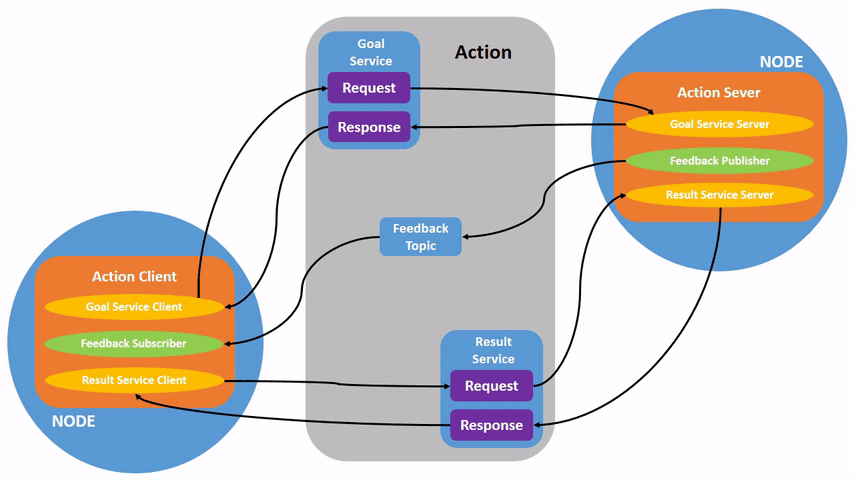
\includegraphics[scale=0.7]{Pictures/Action-SingleActionClient.png}\\
\end{center}
\caption{Action Node en een client node. {\tiny (afbeelding van ros.org)}}\label{fig:action_node}
\end{figure}


\section{Action message structure}
\label{sec:action_message_structure}
Net als bij services moet de structuur van de berichten aangeven worden. Dit doen we in een .action-bestand en wordt in de ROS documentatie een `action' genoemd. In deze reader verwijzen we er naar met de term `action message structure'. In de action message structuur staan de parameters van de \textit{goal request}, van de \textit{result} en van de \textit{feedback}. In het bestand zijn deze onderdelen gescheiden door middel van drie gedachtenstreepjes (-)\footnote{zie: https://nl.wikipedia.org/wiki/Gedachtestreepje}. Met eerst de goal request, daarna de result en als laatste de structuur van de feedback. In codevoorbeeld \ref{code:template-action-bestand} zien we de template voor een action message structure. In codevoorbeeld \ref{code:action-fib-struct} zien we een uitgewerkte action message structure waarbij de goal request bestaat uit een int32, de result uit een vector<int32> en de feedback uit een vector<int32>. Net als bij services en topics beschrijven we per message een struct, dus we kunnen ook meerdere (verschillende) types toekennen aan \'e\'en bericht. 

\begin{lstlisting}[language=C++, caption={Template van een .action-bestand}, firstnumber=0, label={code:template-action-bestand}]
# Goal request
---
# Result
---
# Feedback
\end{lstlisting}

\begin{lstlisting}[language=C++, caption={Het .action-bestand voor een fibonacci-action server.}, firstnumber=0, label={code:action-fib-struct}]
int32 order
---
int32[] sequence
---
int32[] partial_sequence
\end{lstlisting}

\noindent De mogelijke types die kunnen worden gebruikt in de action message structure zijn te vinden op:
\begin{center}
    \url{https://index.ros.org/doc/ros2/Concepts/About-ROS-Interfaces/}
\end{center}

\noindent Net zoals het message type van de publishers/subscribers (zie sectie \ref{sec:message_types}) en de request and response structure van services (zie sectie \ref{sec:srv_messages}) is het mogelijk de action message structure binnen de package te plaatsen, maar ook om deze buiten de package te plaatsen. 

\noindent \textbf{Let op:} Bij het maken van een \textit{.action}-bestand is het verplicht in de naamgeving PascalCase\footnote{zie \url{https://nl.wikipedia.org/wiki/CamelCase}} te gebruiken. ROS zet de \textit{.action} om naar een \textit{.hpp}-bestand met de naam in snake\_case \footnote{zie: \url{https://en.wikipedia.org/wiki/Snake_case}}, waarbij tussen elke kleine letter en hoofdletter van de PascalCase naamgeving nu een onderstrepingsteken (\_) \footnote{ook wel bekent als \textit{underscore}. Zie \url{https://nl.wikipedia.org/wiki/Underscore}} staat. Bijvoorbeeld de action message structure beschreven in \textit{MyCustomAction.action} wordt geïncludeerd met: 
\begin{lstlisting}[language=C++, caption={}, firstnumber=0, label={}]
#include "path/to/folder/my_custom_action.hpp".
\end{lstlisting}

\noindent In sectie \ref{sec:action_meer_bronnen} staan meer bronnen over action message structure. In deze bronnen staat ook hoe je .action-bestanden toevoegd aan je package en hoe je ze vanuit een andere package includeert. 

\section{Action Server}
Een node noemen we een \textit{action server} als het een membervariabele van het type \textit{rclcpp\_action::Server<T>} heeft. Om historische redenen zitten de benodigdheden voor action server en client niet in rclcpp, maar in \textit{rclcpp\_action}. Deze includeren we met:

\begin{lstlisting}[language=C++, caption={}, firstnumber=0, label={}]
#include "rclcpp_action/rclcpp_action.hpp"
\end{lstlisting}

\noindent Met rclcpp\_action kunnen we vervolgens een action server declareren.
Bijvoorbeeld de action server \textit{action\_server\_} met de action message structure \textit{custom\_interfaces::action::Fibonacci}:

\begin{lstlisting}[language=C++, caption={}, firstnumber=0, label={}]
// 'using' allows us to use a shorter word for long types:
using FibAction = custom_interfaces::action::Fibonacci;
// [...]
rclcpp_action::Server<FibAction>::SharedPtr action_server_;"
\end{lstlisting}

Een action server moet drie typen berichten afhandelen: \textit{goal request}, \textit{cancel request} en \textit{accept and execute}. Bij elk bericht hoort ook een taak. De action server moet na het ontvangen van een goal request of een cancel request het verzoek accepteren of weigeren. Bij de ontvangst van een \textit{accept and execute} bericht moet de action server het uitvoeren van de goal starten. Tijdens het uitvoeren van de goal kan de action server feedback sturen naar de action client. Als de goal behaald is of als de goal wordt gecanceld wordt het resultaat gestuurd naar de action client.

Bij het initialiseren van de action server moeten we voor elk type bericht een functie toekennen die het bericht afhandelt. Deze functies hebben verplichte parameters die we bij het initialiseren binden met \textit{std::placeholders}. Het initialiseren doen we met de template-functie \textit{rclcpp\_action::create\_server<T>()} die als template de action message structure heeft. De complete initialisatie van de action server \textit{action\_server\_} in de class \textit{FibActionServer} met de functie \textit{handle\_goal} voor het afhandelen van de goal request, de functie \textit{handle\_cancel} voor het afhandelen van de cancel request en de functie \textit{handle\_accepted} voor het afhandelen van de goal acceptatie en executie ziet er uit als:

\begin{lstlisting}[language=C++, caption={Initialisatie van de action server \textit{action\_sever\_}.}, firstnumber=0, label={code:initialisatie_action_server}]
using namespace std::placeholders;
// 'using' allows us to use a shorter word for long types:
using FibAction = custom_interfaces::action::Fibonacci;
// [...]
this->action_server_ = rclcpp_action::create_server<FibAction>(
    this,
    "fibonacci",
    std::bind(&FibActionServer::handle_goal, this, _1, _2),
    std::bind(&FibActionServer::handle_cancel, this, _1),
    std::bind(&FibActionServer::handle_accepted, this, _1));
\end{lstlisting}

De functies die worden gebonden in tijdens de initialisatie van een \textit{rclcpp\_action::create\_server} hebben net als de functies bij subscribers, service server en service client verplichte parameters en return types. Om de lezer daar bewust van te maken laten we de functie declaraties zien van de gebonden functies in codevoorbeeld \ref{code:initialisatie_action_server}. In de volgende secties bekijken we de inhoud van deze functies.

\begin{lstlisting}[language=C++, caption={De \textit{action\_server\_} functies die de berichten afhandelen.}, firstnumber=0, label={code:action_server_functies}]
// 'using' allows us to use a shorter word for these long types:
using FibAction = custom_interfaces::action::Fibonacci;
using GoalHandleFib = rclcpp_action::ServerGoalHandle<FibAction>;

// [...]

rclcpp_action::GoalResponse handle_goal(
    const rclcpp_action::GoalUUID & uuid, 
    std::shared_ptr<const FibAction::Goal> goal
);

rclcpp_action::CancelResponse handle_cancel(
    const std::shared_ptr<GoalHandleFib> goal_handle
);

void handle_accepted(const std::shared_ptr<GoalHandleFib> goal_handle);
\end{lstlisting}

\subsection{Goal request functie}
\noindent Het speciale return type van  \textit{handle\_goal()} function in codevoorbeeld \ref{code:action_server_functies} geeft de mogelijkheid om terug te geven of de goal wordt geaccepteerd of niet. Dit doet de functie door of \textit{rclcpp\_action::GoalResponse::REJECT} of \textit{rclcpp\_action::GoalResponse::ACCEPT\_AND\_EXECUTE} terug te geven. We zien dit in codevoorbeeld \ref{code:handel_goal}. Let op de functie in codevoorbeeld \ref{code:handel_goal} heeft verplicht twee parameters, maar we gebruiken de parameter \textit{uuid}\footnote{UUID (universally unique identifier) is een manier om (zo goed als) uniqe identifiers te maken. Voor meer informatie: \url{https://en.wikipedia.org/wiki/Universally_unique_identifier}. Of met meer wiskunde: \url{https://towardsdatascience.com/are-uuids-really-unique-57eb80fc2a8}.} niet. Om warnings hiervan te onderdrukken casten we de parameter naar void\footnote{Voor meer informatie over casten naar void: https://stackoverflow.com/questions/34288844/what-does-casting-to-void-really-do}.
\begin{lstlisting}[language=C++, caption={De \textit{handle\_goal()} functie van \textit{action\_server\_}}, firstnumber=0, label={code:handel_goal}]
rclcpp_action::GoalResponse FibActionServer::handle_goal(
    const rclcpp_action::GoalUUID & uuid, 
    std::shared_ptr<const FibAction::Goal> goal
){
    RCLCPP_INFO(this->get_logger(), "Received goal request with order %d", goal->order);
    
    (void)uuid;
    
    // to show an example of rejecting we reject fibonacy sequences that are over 9000:
    if (goal->order > 9000) {
      return rclcpp_action::GoalResponse::REJECT;
    }
    return rclcpp_action::GoalResponse::ACCEPT_AND_EXECUTE;
}
\end{lstlisting}
Als de functie die de goal request afhandelt \textit{ACCEPT\_AND\_EXECUTE} teruggeeft wordt de functie van de action server gebonden aan dit bericht aangeroepen (zie sectie \ref{sec:accept_functie}). Accept and execute is dus een bericht van de action server naar de action client en naar zichzelf. 


\subsection{Cancel request functie}
\noindent Op de zelfde manier als de goal request functie kan de functie die de cancel request afhandelt door middel van \textit{rclcpp\_action::CancelResponse::REJECT} of \textit{rclcpp\_action::CancelResponse::ACCEPT} aangeven of de cancel request wordt geaccepteerd of niet. Als het cancel request is geaccepteerd betekent dat niet dat de goal ook gelijk is gecanceld. Bij het uitvoeren van de goal moet hier dus actief op worden gecontroleerd en de actie ook echt stoppen (zie sectie \ref{sec:accept_functie}). 

\subsection{Accepted en execute functie}
\label{sec:accept_functie}
De functie in de action server node die dit bericht afhandelt start meestal gelijk een andere thread, zodat de node weer nieuwe communicatie kan afhandelen. We zien dit in codevoorbeeld \ref{code:handel_accepted}:

\begin{lstlisting}[language=C++, caption={\textit{handle\_accepted()} start functie execute() in een thread. Hierin wordt de actie uitgevoerd.}, firstnumber=0, label={code:handel_accepted}]
using namespace std::placeholders;
using FibAction = custom_interfaces::action::Fibonacci;
using GoalHandleFib = rclcpp_action::ServerGoalHandle<FibAction>;
// [...]

void FibActionServer::handle_accepted(const std::shared\_ptr<GoalHandleFib> goal\_handle){
    // this needs to return quickly to avoid blocking the executor, so spin up a new thread
    std::thread{std::bind(&FibActionServer::execute, this, _1), goal_handle}.detach();
}
\end{lstlisting}

Tijdens de uitvoering van de action kan de action server feedback sturen naar de action client en als de actie stopt, omdat de goal behaald of is gecanceld, moet het resultaat worden verstuurd. Dit doen we met behulp \textit{rclcpp\_action::ServerGoalHandle<T>}, ook wel de \textit{goal handle} genoemd. Het is daarom belangrijk dat we de goal handle ook meegeven aan de functie die het uitvoeren doet. Dit gebeurt dan ook in codevoorbeeld \ref{code:handel_accepted}. Gegeven de goal handle \textit{goal\_handle} kunnen we de goal opvragen, feedback sturen en het eindresultaat sturen. Zie hiervoor respectievelijk codevoorbeeld \ref{code:goal_handle_getgoal}, \ref{code:goal_handle_sendfeedback} en \ref{code:goal_handle_sendresult}. Vanuit de goal handle kunnen we ook informatie krijgen of een cancel request geaccepteerd is en aangeven dat de goal ook daadwerkelijk gecanceld is. Code hiervoor zien we in codevoorbeeld \ref{code:goal_handle_cancel}.

\begin{lstlisting}[language=C++, caption={Gebruik van de \textit{get\_goal()} functie.}, firstnumber=0, label={code:goal_handle_getgoal}]
const auto goal = goal_handle->get_goal()
\end{lstlisting}

\begin{lstlisting}[language=C++, caption={Het versturen van feedback met een goal handle.}, firstnumber=0, label={code:goal_handle_sendfeedback}]
auto feedback = std::make_shared<FibAction::Feedback>();
auto & sequence = feedback->partial_sequence;
sequence.push_back(0);
sequence.push_back(1);

goal_handle->publish_feedback(feedback);
\end{lstlisting}

\begin{lstlisting}[language=C++, caption={Het versturen van het result met een goal handle.}, firstnumber=0, label={code:goal_handle_sendresult}]
auto result = std::make_shared<FibAction::Result>();
sequence.push_back(0);
sequence.push_back(1);

result->sequence = sequence;
goal_handle->succeed(result);
\end{lstlisting}

\begin{lstlisting}[language=C++, caption={Het controleren op een cancel request acceptatie en de afhandeling daarvan.}, firstnumber=0, label={code:goal_handle_cancel}]
if(goal_handle->is_canceling()) {

    // do, if needed, some actions to really cancel the action goal.

    // set is_cancelling to false again and sends the (incomplete) result:
    goal_handle->canceled(result); // see previous code example for how to make a result
 
    return; // end the current function (and thread)
};
\end{lstlisting}

\subsection{Codevoorbeeld}
In codevoorbeelden \ref{code:action_server_hpp}, \ref{code:action_server_cpp} en \ref{code:action_server_main} zien we alle ingredienten van de action server bij elkaar om een action server node te maken die de fibonacci reeks uitrekent.

\begin{lstlisting}[language=C++, caption={ActionServerNode.hpp}, firstnumber=0, label={code:action_server_hpp}]
#ifndef FIB_ACTION_SERVER_HPP
#define FIB_ACTION_SERVER_HPP

#include "rclcpp/rclcpp.hpp"                // Needed for nodes
#include "rclcpp_action/rclcpp_action.hpp"  // needed for actions

// the location of our custom action.
// the hpp generated by ROS as a underscore (_) before every capital, expect the first:
// for example: /my/path/MyAction.action become /my/path/my_action.action
#include "custom_interfaces/action/fibonacci.hpp"

class FibActionServer : public rclcpp::Node {
public:
    // 'using' allows us to use a shorter word for these long types:
    using FibAction = custom_interfaces::action::Fibonacci;
    using GoalHandleFib = rclcpp_action::ServerGoalHandle<FibAction>;

    FibActionServer();
  
private:
    rclcpp_action::GoalResponse handle_goal(
        const rclcpp_action::GoalUUID & uuid, 
        std::shared_ptr<const FibAction::Goal> goal
    );

    rclcpp_action::CancelResponse handle_cancel(
        const std::shared_ptr<GoalHandleFib> goal_handle
    );

    void handle_accepted(const std::shared_ptr<GoalHandleFib> goal_handle);

    void execute(const std::shared_ptr<GoalHandleFib> goal_handle);

    rclcpp_action::Server<FibAction>::SharedPtr action_server_;
};

#endif /* FIB_ACTION_SERVER_HPP */
\end{lstlisting}

\begin{lstlisting}[language=C++, caption={ActionServerNode.cpp}, firstnumber=0, label={code:action_server_cpp}]
#include "FibActionServer.hpp"
#include "rclcpp/rclcpp.hpp"                // Needed for nodes
#include "rclcpp_action/rclcpp_action.hpp"  // needed for actions

// the location of our custom action.
// the hpp generated by ROS as a underscore (_) before every capital, expect the first:
// for example: /my/path/MyAction.action become /my/path/my_action.action
#include "custom_interfaces/action/fibonacci.hpp"

using namespace std::placeholders;

// constructor:
FibActionServer::FibActionServer(): Node("fibonacci_action_server") {

    this->action_server_ = rclcpp_action::create_server<FibAction>(
        this,
        "fibonacci",
        std::bind(&FibActionServer::handle_goal, this, _1, _2),
        std::bind(&FibActionServer::handle_cancel, this, _1),
        std::bind(&FibActionServer::handle_accepted, this, _1));
}

rclcpp_action::GoalResponse FibActionServer::handle_goal(
    const rclcpp_action::GoalUUID & uuid, // uuid means universally unique identifier
    std::shared_ptr<const FibAction::Goal> goal
){
    RCLCPP_INFO(this->get_logger(), "Received goal request with order %d", goal->order);
    // we are not using the uuid. If you dont use a parameter you will get a warning.
    // the parameters are predefined by ROS, so we cant remove the uuid parameter.
    // So we supress the warning by casting the uuid variable to void:
    (void)uuid;

    // to show an example of rejecting we reject fibonacy sequences that are over 9000:
    if (goal->order > 9000) {
      return rclcpp_action::GoalResponse::REJECT;
    }
    return rclcpp_action::GoalResponse::ACCEPT_AND_EXECUTE;
}

rclcpp_action::CancelResponse FibActionServer::handle_cancel(
    const std::shared_ptr<GoalHandleFib> goal_handle
){
    RCLCPP_INFO(this->get_logger(), "Received request to cancel goal");
    // we are not using the parameter goal_handel
    // to supress warnings we cast it to void:
    (void)goal_handle;
    return rclcpp_action::CancelResponse::ACCEPT;
}

void FibActionServer::handle_accepted(const std::shared_ptr<GoalHandleFib> goal_handle){
    using namespace std::placeholders;
    // this needs to return quickly to avoid blocking the executor, so spin up a new thread
    std::thread{std::bind(&FibActionServer::execute, this, _1), goal_handle}.detach();
}

void FibActionServer::execute(const std::shared_ptr<GoalHandleFib> goal_handle){
    RCLCPP_INFO(this->get_logger(), "Executing goal");

    rclcpp::Rate loop_rate(1); // loop frequency

    const auto goal = goal_handle->get_goal();
    auto feedback = std::make_shared<FibAction::Feedback>();
    auto & sequence = feedback->partial_sequence;
    sequence.push_back(0);
    sequence.push_back(1);
    auto result = std::make_shared<FibAction::Result>();

    for (int i = 1; (i < goal->order) && rclcpp::ok(); ++i) {
        // Check if there is a cancel request
        // is_canceling is true if a cancelling message is send.
        if (goal_handle->is_canceling()) { 
            result->sequence = sequence;
            goal_handle->canceled(result); // set is_cancelling to false again
            RCLCPP_INFO(this->get_logger(), "Goal Canceled");
            return;
        }

        // Update sequence
        sequence.push_back(sequence[i] + sequence[i - 1]);

        // Publish feedback
        goal_handle->publish_feedback(feedback);
        RCLCPP_INFO(this->get_logger(), "Publish Feedback");

        // sleep until next loop (see loop_rate at the start of this function)
        loop_rate.sleep();
    }

    // the goal is done (the for loop ended):
    if (rclcpp::ok()) {
      result->sequence = sequence;
      goal_handle->succeed(result);
      RCLCPP_INFO(this->get_logger(), "Goal Succeeded");
    }
}

\end{lstlisting}

\begin{lstlisting}[language=C++, caption={mainActionServerNode.cpp}, firstnumber=0, label={code:action_server_main}]
#include "FibActionServer.hpp"
#include "rclcpp/rclcpp.hpp"  


int main(int argc, char ** argv)
{
  rclcpp::init(argc, argv);
  
  auto action_server = std::make_shared<FibActionServer>();
  rclcpp::spin(action_server);
  rclcpp::shutdown();
  
  return 0;
}
\end{lstlisting}

\section{Action client}
Een \textit{action client} kan een goal indienen bij een action server. Als deze wordt geaccepteerd, dan krijgt de action client daarvan feedback\footnote{Mits de action server deze stuurt}, en uiteindelijk het het resultaat. Als een goal loopt bij een action server, dan kan een action client ook een cancel request sturen naar de action server.

Een node neemt de communicatierol \textit{action client} op zich door een member variabele te maken van het type \textit{rclcpp\_action::Client<T>}. Waarbij voor de template een action message structure moet worden ingevuld. Bijvoorbeeld met de action message structure \textit{custom\_interfaces::action::Fibonacci}:

\begin{lstlisting}[language=C++, caption={}, firstnumber=0, label={}]
// 'using' allows us to use a shorter word for long types:
using FibAction = custom_interfaces::action::Fibonacci;

//[...]
rclcpp_action::Client<FibAction>::SharedPtr client_ptr_;
\end{lstlisting}

\noindent Het initialiseren van de action client is relatief makkelijk. Met de functie \textit{rclcpp\_action::create\_client<T>()} hebben we enkel de action message structure en de naam van de action nodig. Bijvoorbeeld met de action message structure \textit{custom\_interfaces::action::Fibonacci} en de action naam \textit{fibonacci}:



\begin{lstlisting}[language=C++, caption={}, firstnumber=0, label={}]
using FibAction = custom_interfaces::action::Fibonacci;
//[...]

this->client_ptr_ = rclcpp_action::create_client<FibAction>(
      this,
      "fibonacci");
\end{lstlisting}

\noindent Om een goal te versturen moeten we eerst een goal message maken. Deze maken we met behulp van een functie die ROS ons geeft met de action message structure:

\begin{lstlisting}[language=C++, caption={}, firstnumber=0, label={}]
using FibAction = custom_interfaces::action::Fibonacci;
//[...]

auto goal_msg = FibAction::Goal();
goal_msg.order = 10;
\end{lstlisting}

\noindent Voordat we de goal kunnen versturen moeten we instellen welke functies de berichten van de action server verwerken. Er zijn drie berichten die we terug kunnen krijgen: goal response, feedback en result. De goal response bevat of de action server de goal heeft geaccepteerd of heeft geweigerd. Het binden van functies aan de berichten gaat op een vergelijkbare manier als bij andere rollen. Daarna kunnen we goal versturen met \textit{async\_send\_goal()} van de action client member:

\begin{lstlisting}[language=C++, caption={}, firstnumber=0, label={}]
using namespace std::placeholders;
using FibAction = custom_interfaces::action::Fibonacci;
//[...]

// setting the functions that handle the return-messages:
auto SGO = rclcpp_action::Client<FibAction>::SendGoalOptions();
SGO.goal_response_callback = std::bind(&FibActionClient::goal_response_callback, this,_1);
SGO.feedback_callback = std::bind(&FibActionClient::feedback_callback, this, _1, _2);
SGO.result_callback = std::bind(&FibActionClient::result_callback, this, _1);

// sending the goal:
auto goal_handle_future = this->client_ptr_->async_send_goal(goal_msg, SGO);
\end{lstlisting}

Via de parameters van de functies kunnen we de feedback en result binnen halen. Ook kunnen we via deze parameters meer informatie krijgen over het goal. Bijvoorbeeld of de result die we krijgen een resultaat is dat is ontstaan omdat het goal is behaald of omdat het goal is gecanceld. In sectie \ref{sec:action_client_code} zien we het gebruik hiervan in de codevoorbeelden.

\subsection{Codevoorbeeld}
\label{sec:action_client_code}
In codevoorbeelden \ref{code:action_client_hpp}, \ref{code:action_client_cpp} en \ref{code:action_client_main} zien we alle ingrediënten van de action client bij elkaar om een action client server node te maken die een action server vraagt om een fibonacci reeks uit te rekenen.

\begin{lstlisting}[language=C++, caption={ActionClientNode.hpp}, firstnumber=0, label={code:action_client_hpp}]
#ifndef FIB_ACTION_CLIENT_HPP
#define FIB_ACTION_CLIENT_HPP

#include "rclcpp/rclcpp.hpp"
#include "rclcpp_action/rclcpp_action.hpp"

// the location of our custom action.
// the hpp generated by ROS as a underscore (_) before every capital, expect the first:
// for example: /my/path/MyAction.action become /my/path/my_action.action
#include "custom_interfaces/action/fibonacci.hpp"

class FibActionClient : public rclcpp::Node
{
public:
  // 'using' allows us to use a shorter word for these long types:
  using FibAction = custom_interfaces::action::Fibonacci;
  using GoalHandleFib = rclcpp_action::ClientGoalHandle<FibAction>;

  explicit FibActionClient(const rclcpp::NodeOptions & node_options = rclcpp::NodeOptions());

  // used in the main to stop the client when the goal is done.
  bool is_goal_done() const;

  void send_goal();

private:
  rclcpp_action::Client<FibAction>::SharedPtr client_ptr_;
  rclcpp::TimerBase::SharedPtr timer_;
  bool goal_done_;

  void goal_response_callback(std::shared_future<GoalHandleFib::SharedPtr> future);

  void feedback_callback(
    GoalHandleFib::SharedPtr,
    const std::shared_ptr<const FibAction::Feedback> feedback);

  void result_callback(const GoalHandleFib::WrappedResult & result);

}; 

#endif /* FIB_ACTION_CLIENT_HPP */
\end{lstlisting}

\begin{lstlisting}[language=C++, caption={ActionClientNode.cpp}, firstnumber=0, label={code:action_client_cpp}]
#include <inttypes.h>
#include <memory>
#include <string>
#include <iostream>

#include "rclcpp/rclcpp.hpp"
#include "rclcpp_action/rclcpp_action.hpp"

#include "FibActionClient.hpp"
#include "custom_interfaces/action/fibonacci.hpp"

using namespace std::placeholders; // needed for the _1 and _2 in std::bind

FibActionClient::FibActionClient(const rclcpp::NodeOptions & node_options)
: Node("fib_action_client", node_options), goal_done_(false)
{
    this->client_ptr_ = rclcpp_action::create_client<FibAction>(
      this,
      "fibonacci");

    this->timer_ = this->create_wall_timer(
        std::chrono::milliseconds(500),
        std::bind(&FibActionClient::send_goal, this));
}

bool FibActionClient::is_goal_done() const
{
    return this->goal_done_;
}

void FibActionClient::send_goal()
{
    // cancel the timer.
    this->timer_->cancel();

    // the goal is not done.
    this->goal_done_ = false;

    // wait till the action server is also running.
    if (!this->client_ptr_->wait_for_action_server(std::chrono::seconds(10))) {
        RCLCPP_ERROR(this->get_logger(), "Action server not available after waiting");
        this->goal_done_ = true;
        return;
    }

    // create a new goal message:
    auto goal_msg = FibAction::Goal();
    goal_msg.order = 10;

    // print in logger
    RCLCPP_INFO(this->get_logger(), "Sending goal");
    
    // setting the functions that handle the return-messages:
    auto send_goal_options = rclcpp_action::Client<FibAction>::SendGoalOptions();
    send_goal_options.goal_response_callback = std::bind(&FibActionClient::goal_response_callback, this, _1);
    send_goal_options.feedback_callback = std::bind(&FibActionClient::feedback_callback, this, _1, _2);
    send_goal_options.result_callback = std::bind(&FibActionClient::result_callback, this, _1);

    // sending the goal:
    auto goal_handle_future = this->client_ptr_->async_send_goal(goal_msg, send_goal_options);
}



void FibActionClient::goal_response_callback(std::shared_future<GoalHandleFib::SharedPtr> future)
{
    auto goal_handle = future.get();
    if (!goal_handle) {
        RCLCPP_ERROR(this->get_logger(), "Goal was rejected by server");
    } else {
        RCLCPP_INFO(this->get_logger(), "Goal accepted by server, waiting for result");
    }
}

void FibActionClient::feedback_callback(
    GoalHandleFib::SharedPtr,
    const std::shared_ptr<const FibAction::Feedback> feedback
    ){
    RCLCPP_INFO(
        this->get_logger(), 
        "Next number in sequence received: %" PRId32,
        feedback->partial_sequence.back()
    );
}

void FibActionClient::result_callback(const GoalHandleFib::WrappedResult & result)
{
    this->goal_done_ = true;
    // result.code contains information why the result is send.
    // It is possible to get an incomplete result, for example when the
    // goal is canceled.
    switch (result.code) {
        case rclcpp_action::ResultCode::SUCCEEDED:
            break;
        case rclcpp_action::ResultCode::ABORTED:
            RCLCPP_ERROR(this->get_logger(), "Goal was aborted");
            return;
        case rclcpp_action::ResultCode::CANCELED:
            RCLCPP_ERROR(this->get_logger(), "Goal was canceled");
            return;
        default:
            RCLCPP_ERROR(this->get_logger(), "Unknown result code");
            return;
    }   

    RCLCPP_INFO(this->get_logger(), "Result received");
    for (auto number : result.result->sequence) {
        RCLCPP_INFO(this->get_logger(), "%" PRId32, number);
    }
}
\end{lstlisting}

\begin{lstlisting}[language=C++, caption={mainActionClientNode.cpp}, firstnumber=0, label={code:action_client_main}]
#include "rclcpp/rclcpp.hpp"
#include "FibActionClient.hpp"

int main(int argc, char ** argv)
{
  rclcpp::init(argc, argv);
  auto action_client = std::make_shared<FibActionClient>();

  // Let the client send one goal and then close it:
  while (!action_client->is_goal_done()) {
    rclcpp::spin_some(action_client);
  }

  rclcpp::shutdown();
  return 0;
}
\end{lstlisting}




\section{Meer bronnen:}
\label{sec:action_meer_bronnen}
Een simpele uitleg van wat actions zijn:
\begin{center}
    {\footnotesize \url{https://index.ros.org/doc/ros2/Tutorials/Understanding-ROS2-Actions/}}
\end{center}
\noindent Hoe je je eigen actions maakt:
\begin{center}
    {\footnotesize \url{https://index.ros.org/doc/ros2/Tutorials/Actions/Creating-an-Action/}}
\end{center}
\noindent Hoe je je eigen action client en action server maakt:
\begin{center}
    {\footnotesize \url{https://index.ros.org/doc/ros2/Tutorials/Actions/Writing-a-Cpp-Action-Server-Client/}}
\end{center}




\chapterimage{cc_pixabay_header_robot_on_stairs} 
\chapter{ROS tools en etc.}
In de afbeeldingen \ref{fig:topics} en \ref{fig:service} zien we meerdere nodes en verbindingen die aangeven hoe de nodes met elkaar communiceren. Dergelijke figuren noemen we een \textit{communication graph} van de architectuur van het systeem. Deze type afbeeldingen geven de stroom van informatie aan en welke nodes afhankelijk zijn van welke nodes. Als we naar een groter systeem gaan, zoals te zien in figuur \ref{fig:architectuur-WOR1920-S2}, wordt het lastiger om hier goed overzicht van te houden. Er zijn verschillende manieren om toch overzicht te houden, waaronder de belangrijkste: het modelleren van het systeem. Gelukkig biedt ook ROS 2 hier ons hulpmiddelen bij. Bekijk daarom goed wat er allemaal mogelijk is met ROS via de commandline. Naast de hulpmidellen voor modelleren biedt de ROS 2 commandline commando's ook opties voor testen, analyseren en beheer. In de volgende sectie geven we een zeer incomplete lijst van de mogelijkheden.

\begin{figure}[ht]
\begin{center}
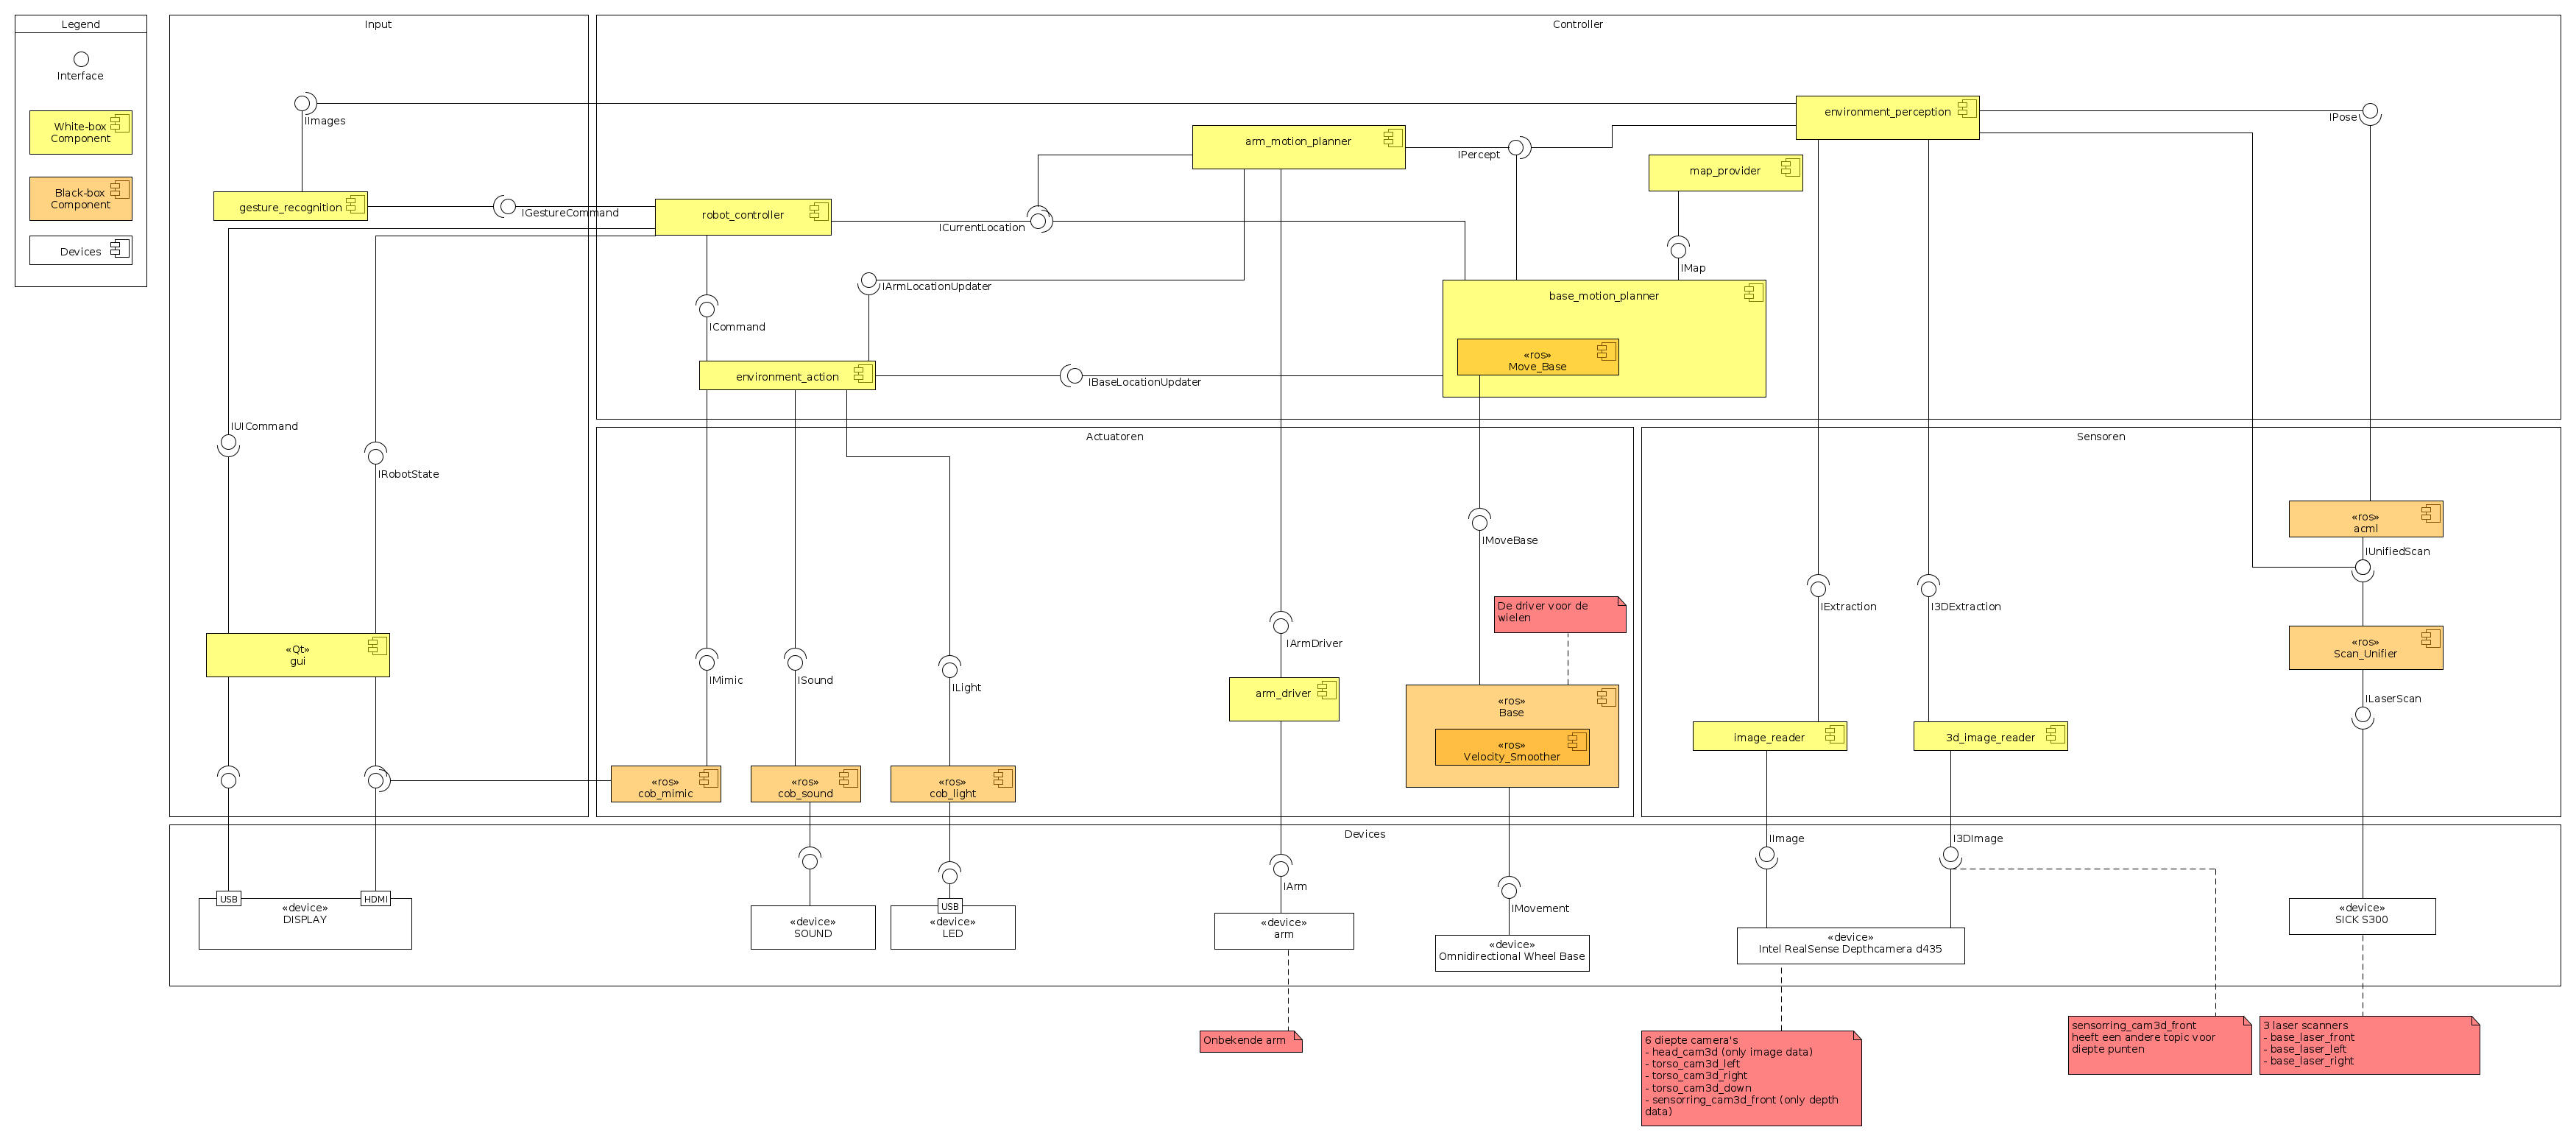
\includegraphics[scale=0.18, angle=-90, origin=c]{architectuur-WOR1920-S2}\\
\end{center}
\caption{De architectuur van het \textit{World Of Robots}-project van 19-20 S2 bij de opleiding ESD aan de HAN.}\label{fig:architectuur-WOR1920-S2}
\end{figure}

\section{Handige ROS commando's}
ROS komt allerlei handige commando's om je packages te bouwen en te onderhouden. In table \ref{table:ROS_commandos} staan er een aantal. Weet jij een commando die hier aan moet worden toegevoegd, neem dan vooral contact op met de auteur. 

\begin{table}[h]
\centering
\rowcolors{2}{green!95!yellow!50}{green!65!yellow!40}
\setlength{\arrayrulewidth}{0.5mm}
\setlength{\tabcolsep}{9pt}
\renewcommand{\arraystretch}{1.5}

\begin{tabular}{|l|l|}
\hline
\textbf{COMMAND}               & \textbf{RESULTAAT}                                \\ \hline
ros2 topic hz /[topic\_name]    & Geeft de frequentie statistieken van een topic.                                         \\ \hline
rqt\_graph                       & laat alle actieve nodes en communicatie zien      \\ \hline
\multicolumn{2}{|l|}{\textbf{ACTIONS}}                                                \\ \hline
ros2 action list                & Geeft alle actions in de ROS graph                \\ \hline
ros2 action info <action>       & Geeft het aantal clients en servers voor de action.\\ \hline
          &                     \\ \hline
\end{tabular}
\caption{Een incomplete lijst met handige ROS 2 commando's.}
\label{table:ROS_commandos}
\end{table}

\section{Achtergrond}
Diepere uitleg over ROS 2 en de gemaakte designkeuzes zijn onder andere te vinden op: \\
\begin{center}
    \url{https://design.ros2.org/}
\end{center}


\chapterimage{cc_pixabay_header_package} 
\chapter{ROS packages}
ROS komt met een aantal handige packages (libraries) die het werken met en het programmeren van robots makkelijker maken. In dit hoofdstuk kijken we naar de transform library bekent als tf2\footnote{\url{https://wiki.ros.org/tf2} ; Pas op: de meeste voorbeelden op deze link zijn met ROS 1.}

\section{Tf2}
Tf2  (\underline{t}rans\underline{f}orm library 2) is een ROS package (library) die helpt bij het omrekenen van verschillende coördinatensystemen naar elkaar. Dit is erg handig als we werken met hardwarecomponenten die moet samenwerken in de echte wereld. Deze sectie beschrijft wanneer je tf2 nodig hebt en hoe je tf2 gebruikt.

\subsection{Meerdere coördinatensystemen}
Elk hardwarecomponent dat interacteert met de wereld heeft zijn eigen \textit{coordinate frame of reference} of kortweg \textit{coordinate frame}. Hiermee bedoelen we dat elk hardwarecomponent zijn eigen nulpunt (referentiekader) heeft waar vanuit hij redeneert waar andere objecten staan. Zo zal een robotarm die op de HAN in Arnhem waarschijnlijk zeggen dat zijn middelpunt\footnote{Midden- versus middel-: \url{https://www.schrijfwijzer.nl/taalvragen/verwarwoordenboek/verwarwoord/362/middel-midden}} van zijn base de coordinaten (0, 0, 0) heeft. Hiermee bedoelen we dat zijn coordinate frame op het middelpunt van zijn frame zit. Deze locatie van de coordinate frame is logisch voor de robotarm, maar onlogisch voor de rest van de wereld. Zeker als de arm schuin op een tafel is bevestigd op GPS coordinaten (51.98673585896382, 5.951850752998225) en op Rijksdriehoekcoördinaten\footnote{zie voor informatie over Rijksdriehoekcoördinaten: \url{https://nl.wikipedia.org/wiki/Rijksdriehoeksco\%C3\%B6rdinaten}. GPS en Rijksdriehoekcoördinaten hebben ieder ook een andere referentiekader.} (193787, 444411). Het werken met een coordinate frame voor een robotarm maakt veel dingen makkelijker. De robotarm hoeft niet te achterhalen waar in de wereld het is. Alles wat het moet doen kan worden beredeneert vanuit zijn eigen locatie. 

Deze egoïstische kijk van een component op coordinate frames geven wel uitdagingen als er meerdere hardwarecomponenten zijn die moeten samenwerken. Elk hardwarecomponenten heeft namelijk zijn eigen coordinate frame en dus een eigen nulpunt. De coördinaten waar een sensor een object ziet komt dan niet overeen met de coördinaten waar de robotarm heen moet bewegen om het object aan te raken. Dit wordt nog ingewikkelder als we de oriëntatie (Pitch, Yaw en Roll) ook meenemen. Sensors en actuatoren staan vaak in verschillende hoeken. Maar het kan erger. Het is ook mogelijk dat de locatie van een coordinate frame in de echte wereld steeds verandert. Bijvoorbeeld bij een sensor bevestigt op de ``hand'' van een robotarm.

Tf2 helpt ons met het managen van de vele coordinate frames die een robot kan hebben. Het geeft de mogelijkheid om coordinate frames van de verschillende (bewegende) onderdelen naar elkaar of naar een gezamelijke coordinate frame (veelal \textit{world frame} genoemd) om te zetten. In figuur \ref{fig:coordinateframes} zien we een robot met verschillende coordinate frames. De groene, blauwe en rode cilinders  geven de oriëntatie en locaties van de (nulpunten) van de verschillende coordinate frames aan.

\begin{figure}[ht]
\begin{center}
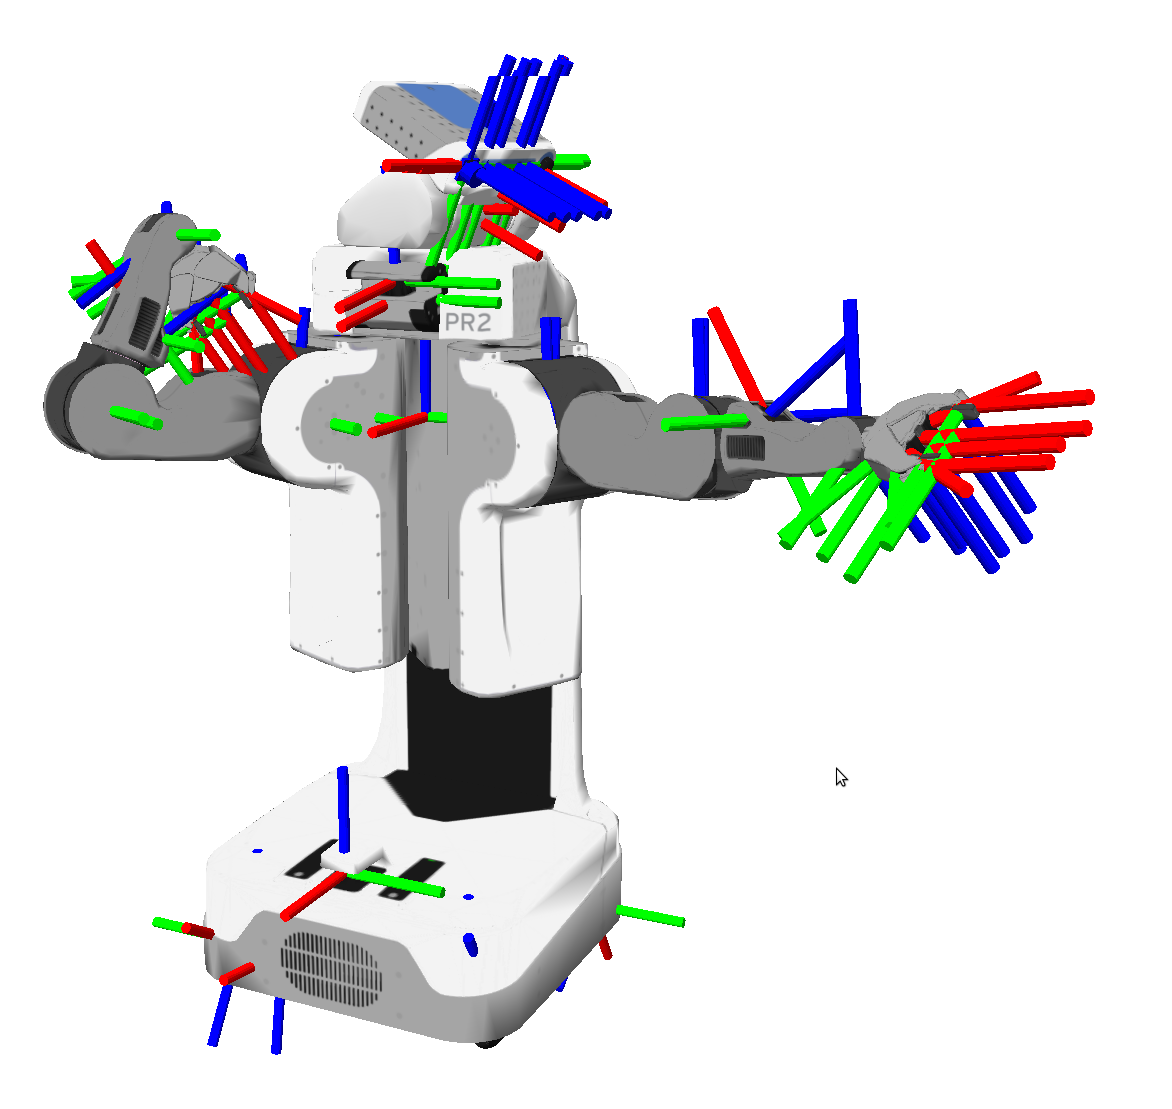
\includegraphics[scale=0.2]{Pictures/robot_multiple_coordinatesystems.png}\\
\end{center}
\caption{Een robot met meerdere coordinate frames met verschillende referentiekaders. De groene, blauwe en rode cilinders  geven de oriëntatie en locaties van de (nulpunten) van de verschillende coordinate frames aan. \tiny{(bron: \url{https://wiki.ros.org/tf2} \cite{tf2-frames})}}
\label{fig:coordinateframes}
\end{figure}

\subsection{Broadcasters en TransformStamped messages}
Tf2 helpt ons bij het communiceren van over welke frames we hebben en wat de relatie is tussen de verschillende frames. Dit doen we door middel van \textit{TransformStamped messages}, \textit{broadcasters} en \textit{listeners}. De TransformStamped messages bevatten de informatie over de frames. Een broadcaster publisheert de TransformStamped messages en een listener geeft ons vervolgens de mogelijkheid om de locatie van elke frame te krijgen in het coordinaten stelsel van een andere frame. De listener leggen we uit in sectie \ref{sec:listeners}.

Er zijn twee verschillende broadcasters: gewone \textit{broadcasters} en \textit{static broadcasters}. De static broadcaster geeft performance voordelen als we deze gebruiken voor frames die weinig of nooit veranderen. In codevoorbeeld \ref{code:frameBroadcaster.hpp} zien we de header file van een ROS node class die twee broadcasters heeft als members. 

\begin{lstlisting}[language=C++, caption={frameBroadcaster.hpp; Een node met twee broadcasters. De twee frames maken samen een 1 DOF-robotarm (zie figuur \ref{fig:1DOFRobotarm} en source file in codevoorbeeld \ref{code:frameBroadcaster.cpp}.}, firstnumber=0, label={code:frameBroadcaster.hpp}]
#ifndef _FRAMEBROADCASTER_H_
#define _FRAMEBROADCASTER_H_

#include "rclcpp/rclcpp.hpp"
#include <tf2_ros/transform_broadcaster.h>
#include <tf2_ros/static_transform_broadcaster.h>

class MinimalTF2Broadcaster : public rclcpp::Node
{
public:
  MinimalTF2Broadcaster();
  
private:
    void createArmFrame();
 
    void moveBase();

    rclcpp::TimerBase::SharedPtr timer_;

    tf2_ros::TransformBroadcaster br;
    tf2_ros::StaticTransformBroadcaster sbr;

    double baseAngle_;
};

#endif

\end{lstlisting}

\noindent Voordat de broadcasters een frame kunnen versturen moet dit in een TransformStamped messages worden gestopt. Een TransformStamped message van een frame heeft de volgende velden:
\begin{itemize}
    \item \textbf{header.stamp:} bevat het tijdstip dat de nieuwe frame waar is. Kan worden gebruikt om terug te kijken in de tijd.
    \item \textbf{header.frame\_id:} ook wel parent frame genoemd. We beschrijven in deze message de locatie en orientatie van de frame in de parent frame.
    \item \textbf{child\_frame\_id:} De naam van deze frame.
    \item \textbf{transform.translation.x:} x-coördinaat van het nulpunt van deze frame in de parent frame.
    \item \textbf{transform.translation.y:} y-coördinaat van het nulpunt van deze frame in de parent frame.
    \item \textbf{transform.translation.z:} z-coördinaat van het nulpunt van deze frame in de parent frame.
    \item\textbf{ transform.rotation.x:} x-Quaternion\footnote{Quaternions zijn een manier om de orientatie in een 3D ruimte te beschrijven. Quaternion zijn fijner in gebruik in computerprogramma's. Zie voor meer informatie: \url{https://nl.wikipedia.org/wiki/Quaternion}} van het nulpunt van deze frame ten opzichte van de parent frame.
    \item \textbf{transform.rotation.y:} y-Quaternion van het nulpunt van deze frame ten opzichte van de parent frame.
    \item \textbf{transform.rotation.z:} z-Quaternion van het nulpunt van deze frame ten opzichte van de parent frame.
    \item \textbf{transform.rotation.w:} w-Quaternion van het nulpunt van deze frame ten opzichte van de parent frame.
\end{itemize}
\noindent In codevoorbeeld \ref{code:frameBroadcaster.cpp} zien we de bijbehorende source file van de header file van codevoorbeeld \ref{code:frameBroadcaster.hpp}. In deze source file wordt er een TransformStamped message gemaakt in de functie \textit{createArmFrame()} en in functie \textit{MoveBase()}. De twee frames beschrijven samen een 1 DOF robotarm (zie figuur. \ref{fig:1DOFRobotarm}). De base frame heeft een locatie en oriëntatie in de world frame. De arm frame heeft een locatie en oriëntatie in de base frame. Indirect heeft hiermee de arm frame ook een locatie en orientatie in de world frame. De functie MoveBase() laat de base frame ronddraaien (als een continuous servo). het ronddraaien van de base zorgt er voor dat de arm frame op een andere locatie is in de world frame. De locatie van de arm frame in de base frame blijft echter hetzelfde!

\begin{figure}[ht]
\begin{center}
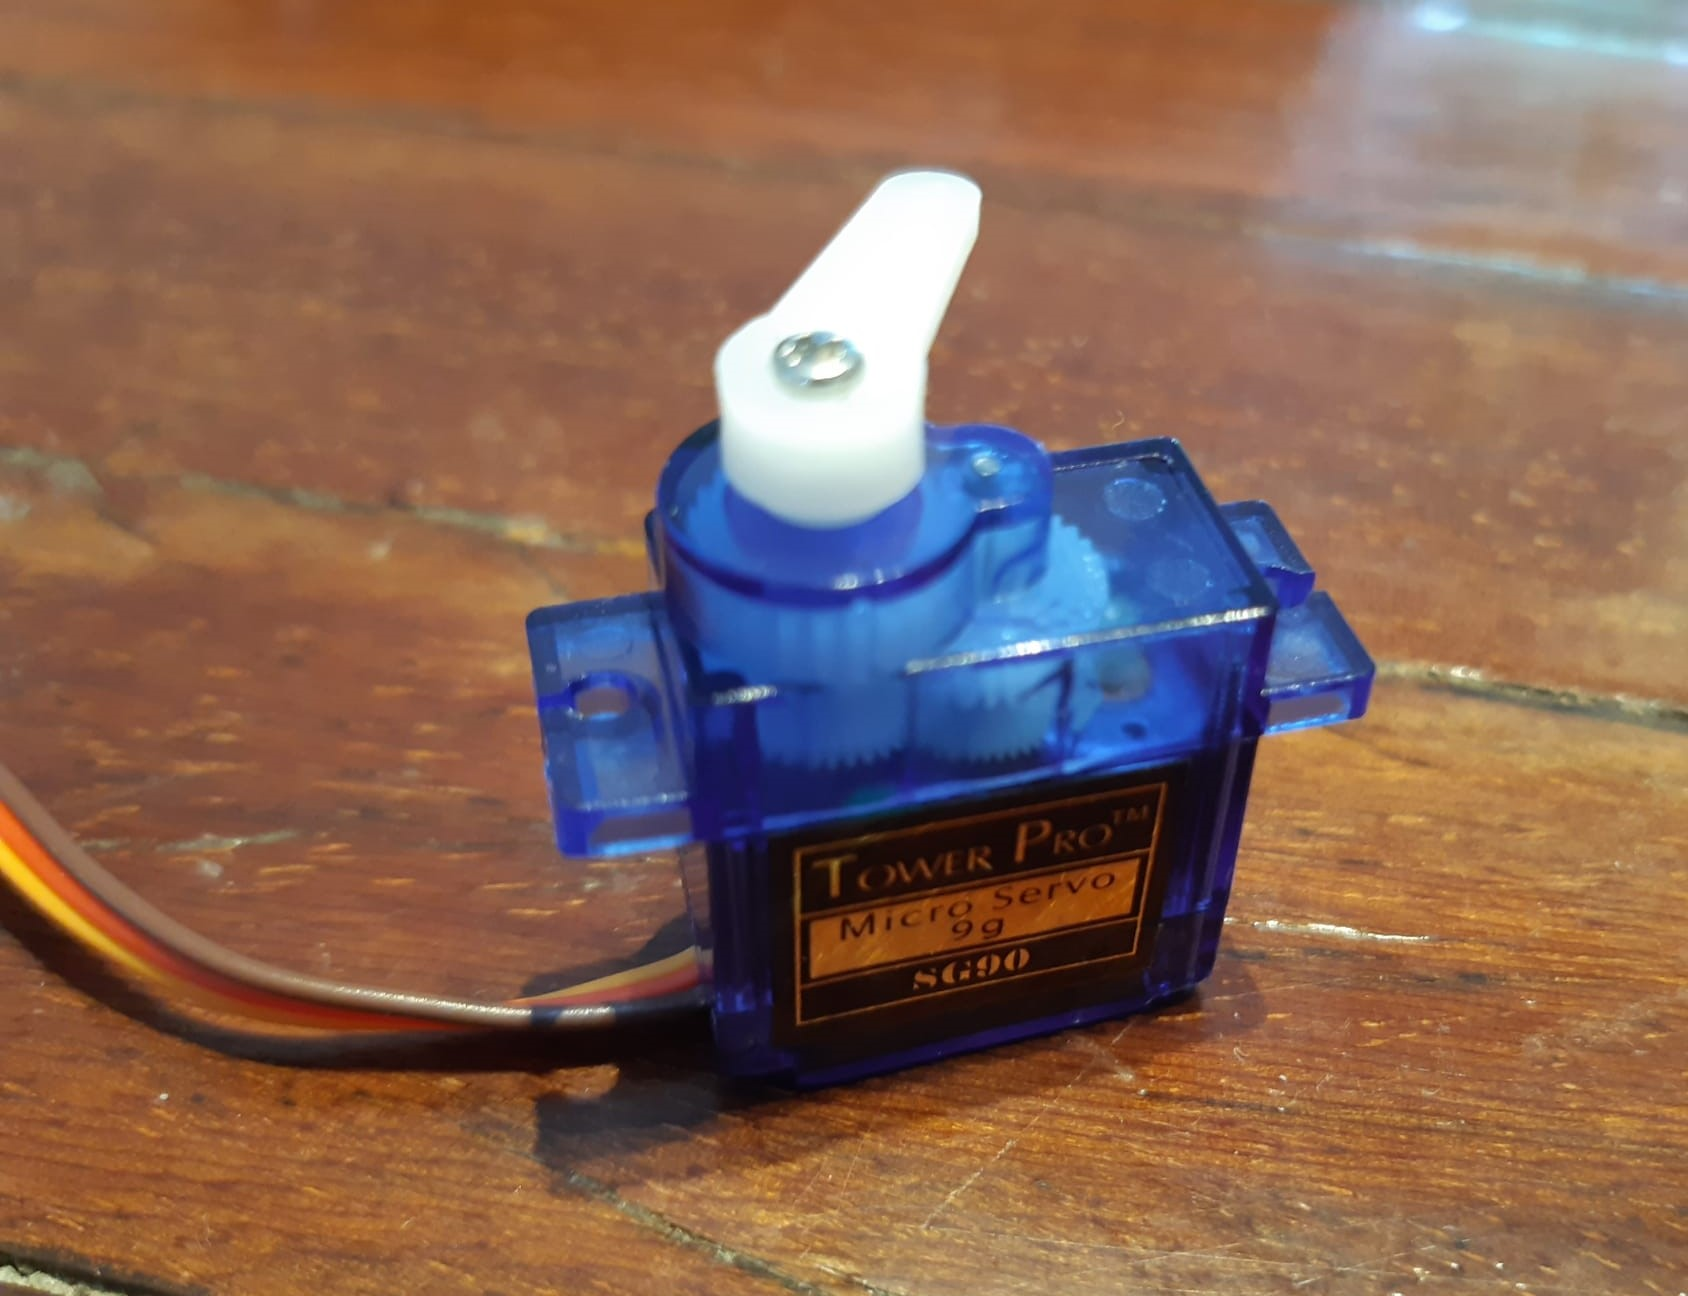
\includegraphics[scale=0.15]{Pictures/servo.jpg}\\
\end{center}
\caption{De 1 DOF robotarm. Codevoorbeeld \ref{code:frameBroadcaster.cpp} maakt een frame genaamd 'base' op de locatie van de schroef. Deze kan dus ronddraaien relatief tot de wereld. De frame 'arm' uit codevoorbeeld \ref{code:frameBroadcaster.cpp} zit aan het uiteinde van het witte armpje dat vast zit aan de 'base'.}
\label{fig:1DOFRobotarm}
\end{figure}

\begin{lstlisting}[language=C++, caption={frameBroadcaster.hpp; Een node met twee broadcasters. De twee frames maken samen een 1 DOF-robotarm (zie figuur \ref{fig:1DOFRobotarm}). De base frame definieert zichzelf met een locatie en oriëntatie in relatie tot de world frame. De arm frame doet dit ook, maar dan in relatie tot de base frame.}, firstnumber=0, label={code:frameBroadcaster.cpp}]
#include "frameBroadcaster.hpp"

#include <chrono>

#include "rclcpp/rclcpp.hpp"
#include <tf2_ros/transform_broadcaster.h>
#include <tf2_ros/static_transform_broadcaster.h>
#include <geometry_msgs/msg/transform_stamped.h>
#include <tf2/LinearMath/Quaternion.h>

using namespace std::chrono_literals;

MinimalTF2Broadcaster::MinimalTF2Broadcaster()
  : Node("MinimalTF2Broadcaster"), br(this), sbr(this), baseAngle_(0)
{
    timer_ = this->create_wall_timer(
    500ms, std::bind(&MinimalTF2Broadcaster::moveBase, this));

    createArmFrame()
}

void MinimalTF2Broadcaster::createArmFrame(){:
    geometry_msgs::msg::TransformStamped static_transformStamped;

    static_transformStamped.header.stamp = this->now();
    static_transformStamped.header.frame_id = "base";
    static_transformStamped.child_frame_id = "arm";
    
    static_transformStamped.transform.translation.x = 0;
    static_transformStamped.transform.translation.y = 5;
    static_transformStamped.transform.translation.z = 0.0;

    tf2::Quaternion q;
    q.setRPY(0, 0, 0); // it is easier for humans to think in roll, pitch and yaw.
    static_transformStamped.transform.rotation.x = q.x();
    static_transformStamped.transform.rotation.y = q.y();
    static_transformStamped.transform.rotation.z = q.z();
    static_transformStamped.transform.rotation.w = q.w();

    sbr.sendTransform(static_transformStamped);
}

void MinimalTF2Broadcaster::moveBase()
{
    // change the rotation of the base:
    baseAngle_ += 0.1;

    geometry_msgs::msg::TransformStamped transformStamped;

    transformStamped.header.stamp = this->now();
    transformStamped.header.frame_id = "world";
    transformStamped.child_frame_id = "base";

    transformStamped.transform.translation.x = 5;
    transformStamped.transform.translation.y = 2;
    transformStamped.transform.translation.z = 0.0;

    tf2::Quaternion q;
    q.setRPY(0, 0, baseAngle_); // it is easier for humans to think in roll, pitch and yaw.
    transformStamped.transform.rotation.x = q.x();
    transformStamped.transform.rotation.y = q.y();
    transformStamped.transform.rotation.z = q.z();
    transformStamped.transform.rotation.w = q.w();

    br.sendTransform(transformStamped);
}

\end{lstlisting}

\subsubsection{Broadcasters testen}
\label{sec:broadcastersTesten}
Als we \'e\'en of meerdere frames hebben aangemaakt kunnen we deze testen met Rviz of met tf2\_echo. Met Rviz kunnen we de locaties, orientaties en relaties van de frames visualiseren. Het gebruik van Rviz kan men vinden in de ROS2 documentatie. We laten hier de de simpelere test met Tf2\_echo zien. Tf2\_echo geeft ons de locatie en oriëntatie van een frame in het stelsel van een andere frame. Om codevoorbeelden \ref{code:frameBroadcaster.hpp} en \ref{code:frameBroadcaster.cpp} te testen kunnen we kijken waar de arm frame zich bevind in de world frame. We doen dat door de node te runnen en in de een andere terminal het volgende uit te voeren\footnote{Het complete voorbeeld in een werkende package is te vinden in de .zip met voorbeelden.}:

\begin{lstlisting}[style=DOS, caption={}, firstnumber=0, label={}]
ros2 run tf2_ros tf2_echo world arm
\end{lstlisting}

\noindent Als de code goed werkt zien we dat de locatie van de arm steeds veranderd\footnote{De x-coördinaat loopt van 0 tot 10 en de y-coordinaat van -3 tot 7}\footnote{nog even kijken of de code in de voorbeelden niet is geupdate. Ik dacht dat hier iets mee was.}. We kunnen ook testen of inderdaad de arm frame wel gelijk blijft in relatie tot de base frame:

\begin{lstlisting}[style=DOS, caption=Hello world, firstnumber=0, label={}]
ros2 run tf2_ros tf2_echo base arm
\end{lstlisting}

\noindent Maar we kunnen de zaken ook van de andere kant bekijken. Soms wil juist vanuit het component redeneren in plaats vanuit de wereld. Je kan dus ook vragen waar het nulpunt van de world is in het coördinaten stelsel van de arm frame:

\begin{lstlisting}[style=DOS, caption=Hello world, firstnumber=0, label={}]
ros2 run tf2_ros tf2_echo arm world
\end{lstlisting}


\subsection{Listeners}\label{sec:listeners}
In sectie \ref{sec:broadcastersTesten} zien we hoe we met een command in de terminal de locatie en oriëntatie van een frame in een andere frame kunnen zien. Dit willen we natuurlijk ook in onze code kunnen doen. Hiervoor gebruiken we de \textit{listeners} van tf2. Listeners krijgen transformStamped messages binnen waarin de locatie en oriëntatie zit van een frame in het stelsel van een andere frame. In codevoorbeeld \ref{code:frameListener.hpp} zien we een de .hpp van een node class die een listener heeft. Naast de listener heeft de node ook een buffer als member. De listener maakt gebruikt van deze buffer. In codevoorbeeld \ref{code:frameListener.cpp} zien we de source van deze node. In de constructor (en specifiek de initializer lists) zien we het declareren van de buffer en de listener. In \textit{listenAndPrint()} wordt de TransformStamped van de arm frame in relatie tot de world frame opgehaald en geprint op het scherm.

\begin{lstlisting}[language=C++, caption={frameListener.hpp; De header file van een node met een listener.}, firstnumber=0, label={code:frameListener.hpp}]
#ifndef _FRAMElISTENER_H_
#define _FRAMElISTENER_H_

#include "rclcpp/rclcpp.hpp"
#include <tf2_ros/transform_listener.h>
#include <tf2_ros/buffer.h>

class MinimalTF2Listener : public rclcpp::Node
{
public:
    MinimalTF2Listener();

private:

    void listenAndPrint();

    rclcpp::TimerBase::SharedPtr timer_;

    tf2_ros::Buffer tfBuffer;
    tf2_ros::TransformListener tfListener;
};

#endif

\end{lstlisting}


\begin{lstlisting}[language=C++, caption={frameListener.hpp; De header file van een node met een listener.}, firstnumber=0, label={code:frameListener.cpp}]
#include "frameListener.hpp"

#include <chrono>

#include "rclcpp/rclcpp.hpp"
#include <tf2_ros/transform_listener.h>
#include <tf2_ros/buffer.h>
#include <geometry_msgs/msg/transform_stamped.h>
#include <tf2/LinearMath/Quaternion.h>

using namespace std::chrono_literals;

MinimalTF2Listener::MinimalTF2Listener()
    : Node("MinimalTF2Listener"), tfBuffer(this->get_clock()), tfListener(tfBuffer)
{
    timer_ = this->create_wall_timer(
        500ms, std::bind(&MinimalTF2Listener::listenAndPrint, this));    
}


void MinimalTF2Listener::listenAndPrint()
{
    geometry_msgs::msg::TransformStamped transformStamped;

    
    try{ // try to get the coordinates of arm in the world frame:
        transformStamped = tfBuffer.lookupTransform("world", "arm", tf2::TimePoint());
    }
    // otherwise explain what went wrong and exit this function:
    catch (const tf2::TransformException & ex) {
        std::cout << "Failure at " << this->now().seconds() << std::endl;
        std::cout << "Exception thrown:" << ex.what() << std::endl;
        std::cout << "The current list of frames is:" << std::endl;
        std::cout << tfBuffer.allFramesAsString() << std::endl;
        return;
    }

    RCLCPP_INFO(this->get_logger(), "The arm is at: (%.5f,%.5f,%.5f)", 
                    transformStamped.transform.translation.x,
                    transformStamped.transform.translation.y,
                    transformStamped.transform.translation.z);
}



\end{lstlisting}

\subsection{Meer informatie:}
De tutorials van tf2 met ROS 2 zijn nog erg minimalistics\footnote{\url{https://index.ros.org/doc/ros2/Tutorials/tf2/}}. Gelukkig is de werking van tf2 niet verandert met de overgang van ROS 1 naar ROS 2. De ROS 1 informatie van tf2 is ook voor ROS2 een goede bron. Let wel op: ROS 1 heeft een andere manier van het maken en opstarten van nodes. Op de onderstaande link vind je meer informatie over tf2:

\begin{center}
    \url{https://wiki.ros.org/tf2}
\end{center}


\section{Rviz} \label{sec:rviz}
In de voorbeelden .zip is een werkend voorbeeld met Rviz te vinden. 
\chapterimage{cc_pixabay_header_backpacker} 
\chapter{Practicum}

\begin{exercise}[Nom nom nom]\mbox{}\\
Bekijk de onderstaande code en beantwoord de volgende vraag zonder de code uit te voeren op je computer:
\begin{enumerate}
    \item Als de node wordt gestart. Welke naam heeft de node dan in ROS?
    % Het antwoord op de onderstaande vraag is wat ingewikkelder dan ik dacht en er blijken meerdere oplossing ervoor zijn mogelijk. Daarom de vraag weg gehaald.
    %\item De main start nu \'e\'en \textit{VoedselNode}. Is het ook mogelijk om twee \textit{VoedselNode}'s te starten in ROS? 
        %\begin{itemize}
        %    \item Zo nee, wat moeten we aanpassen aan de code om dat wel mogelijk te maken?
        %    \item Zo ja, aan welke eisen voldoet de node waardoor dit mogelijk is?
        %\end{itemize}
\end{enumerate}


\begin{minipage}{0.9\linewidth}
\begin{lstlisting}[language=C++, firstnumber=0]
#include "rclcpp/rclcpp.hpp"

class VoedselNode : public rclcpp::Node
{
public:
    VoedselNode();
};

\end{lstlisting}
\end{minipage}

\begin{minipage}{0.9\linewidth}
\begin{lstlisting}[language=C++, firstnumber=0]
#include "rclcpp/rclcpp.hpp"
#include "VoedeselNode.h"

HelloNode::VoedselNode() : Node("Appelkoek"){
    RCLCPP_INFO(this->get_logger(), "Hallo, ik ben Voedsel!");
}
\end{lstlisting}
\end{minipage}

\begin{minipage}{0.9\linewidth}
\begin{lstlisting}[language=C++, firstnumber=0]
#include "rclcpp/rclcpp.hpp"
#include "VoedselNode.hpp"

int main(int argc, char **argv){
    rclcpp::init(argc, argv);
    auto node = std::make_shared<VoedselNode>();
    rclcpp::spin(node); 
    rclcpp::shutdown(); 
    return 0;
}
\end{lstlisting}
\end{minipage}
% antwoorden:
% 1. "appelkoek"
% 2. De constructor van VoedselNode moet een string meekrijgen die we vervolgens meegeven aan 
\end{exercise}

\newpage

\begin{exercise}[Constructieve communicatie]\mbox{}\\
Bekijk de onderstaande code en beantwoord de volgende vragen zonder de code uit te voeren op je computer:
\begin{enumerate}
\item Wat doet de functie \textbf{std::bind()}?
\item Waarom hebben \textit{using std::placeholders::\_1;} nodig?
\item Als we ArchitectNode en BuilderNode (op volgende pagina) runnen wat zien we dan in de terminal verschijnen?
\item ArchitectNode deelt nu drie designs en wacht na het geven van een design even. We willen dat de node tussen elk design 10 seconden wacht. Welke regel moet worden aangepast en wat is de aanpassing?
\item De nodes maken gebruikt van een custom message. Schrijf de custom message.
\end{enumerate}

\begin{minipage}{0.9\linewidth}
\begin{lstlisting}[language=C++, firstnumber=0]
#include "rclcpp/rclcpp.hpp"
#include "ArchitectNode.h"

ArchitectNode::ArchitectNode(): Node("Djoser"){
    publisher_ = this->create_publisher<nijl::msg::design>("designs", 10);

    rclcpp::Rate timer(0.5);
    shareDesign("*", 3);
    timer.sleep();
    shareDesign("#", 7);
    timer.sleep();
    shareDesign("+", 5);
}

void ArchitectNode::shareDesign(std::string pattern, unsigned int n){
  auto message = nijl::msg::design();
  message.pattern = pattern;
  message.n = n;
  publisher_->publish(message);
}
\end{lstlisting}
\end{minipage}

\begin{minipage}{0.9\linewidth}
\begin{lstlisting}[language=C++, firstnumber=0]
#include "rclcpp/rclcpp.hpp"
#include "BuilderNode.h"
#include <string>

using std::placeholders::_1;

BuilderNode::BuilderNode(): Node("Pat en Mat"){
  subscription_ = this->create_subscription<nijl::msg::design>(
    "designs", 10, std::bind(&BuilderNode::designReceiver, this, _1));
}

void BuilderNode::topic_callback(const Nijl::msg::Design::SharedPtr msg) const
{
  unsigned int n = msg->n;
  std::string floor = "";
  for(unsigned int i=0; i < n; i++){
    floor = "";
    for(unsigned int j=0; j < i; j++){
        floor += msg->pattern;
    }
    RCLCPP_INFO(this->get_logger(), floor.c_str());
  }
  for(unsigned int i=n-1; i >= 0; i--){
    floor = "";
    for(unsigned int j=0; j < i; j++){
        floor += msg->pattern;
    }
    RCLCPP_INFO(this->get_logger(), floor.c_str());
  }
}
\end{lstlisting}
\end{minipage}
 % De bedoeling was  een "driehoek"/"pyramide" van sterretjes van 3 hoog dan van #'s 7 hoog en dan van plusjes 5 hoog, echter niet goed gerealiseerd dat RCLCPP_INFO ook een newline neerzet. Resultaat is dus een hele reeks sterretjes, dan een hele reeks #'s en dan een reeks plusjes.
 % de rclcpp::rate timer moet naar 0.1
 % String \n Int64
 % 
\end{exercise}
% YYYYYYYYYYYYYYYYYYYYYYY
% NEWPAGE!!!!!!!!!!!!!
\newpage
% YYYYYYYYYYYYYYYYYYYYYYY
% NEWPAGE!!!!!!!!!!!!!

\begin{exercise}[Interne conversatie]\mbox{}\\
Bekijk de onderstaande code en beantwoord de volgende vragen zonder de code uit te voeren op je computer:
\begin{enumerate}
\item Wat staat er na het starten van de WeirdNode op het scherm?
%Wat heb je?
%Wat heb je
%Wat heb j
%Wat heb 
%Wat heb
%Wat h
%etc.
\item Wat gebeurd er als we twee WeirdNodes starten?
%afhankelijk van timing, waarschijnlijk:%
%%Wat heb je?
%%Wat heb je?
%Wat heb je (4 keer)
%Wat heb j (8 keer)
%Wat heb (16 keer)
%etc.

\end{enumerate}

\begin{minipage}{0.9\linewidth}
\begin{lstlisting}[language=C++, firstnumber=0]
#include "rclcpp/rclcpp.hpp"
#include "std_msgs/msg/string.hpp"
#include "WeirdNode.h"

using std::placeholders::_1; 

WeirdNode::WeirdNode(const std::string & name): Node(name){
    publisher_ = this->create_publisher<std_msgs::msg::String>("topic", 10);

    subscription_ = this->create_subscription<std_msgs::msg::String>(
    "topic", 10, std::bind(&WeirdNode::topic_callback, this, _1));

    std::string content = "Wat heb je?";
    publishMessage(content);
}

void WeirdNode::topic_callback(const std_msgs::msg::String::SharedPtr msg) const {
    std::string content = msg->data.c_str();
    RCLCPP_INFO(this->get_logger(), "I heard: '%s'", content.c_str());

    if(content.size() > 1){:
        std::string new_content = content.substr(0, content.size()-1);
    
        for(int i=0; i<1000000000; i++){} // wait a bit.

        publishMessage(new_content);
    }
}

void WeirdNode::publishMessage(std::string content) const{
    auto message = std_msgs::msg::String();
    message.data = content;
    publisher_->publish(message);
}
\end{lstlisting}
\end{minipage}

\begin{minipage}{0.9\linewidth}
\begin{lstlisting}[language=C++, firstnumber=0]
#include "rclcpp/rclcpp.hpp"
#include "WeirdNode.h"

int main(int argc, char * argv[])
{
  rclcpp::init(argc, argv);
  rclcpp::spin(std::make_shared<WeirdNode>("Weirdo"));
  rclcpp::shutdown();
  return 0;
}
\end{lstlisting}
\end{minipage}

\end{exercise}

\newpage %!!!!!!!!!!!!!newpage!!!!!!!!!!!!!

\begin{exercise}[Abacus]\mbox{}\\
\begin{minipage}{0.6\textwidth}
Maak een package met twee ROS nodes: één publisher en één subscriber. De publisher schrijft elke 2 seconden een willekeurig cijfer op een topic. De subscriber ontvangt drie berichten van het topic en telt deze bij elkaar op. Het resultaat print de subscriber via de logger. De subscriber print dus elke 6 seconden een resultaat. Als de subscriber later start dan de publisher, dan begint de subscriber bij het eerste bericht dat hij ontvangt via het topic (dit is het standaard gedrag van een subscriber).

Zorg er voor dat je package voldoet aan de conventies van ROS2.
\end{minipage}\hfill 
\begin{minipage}{0.3\textwidth}
\begin{center}
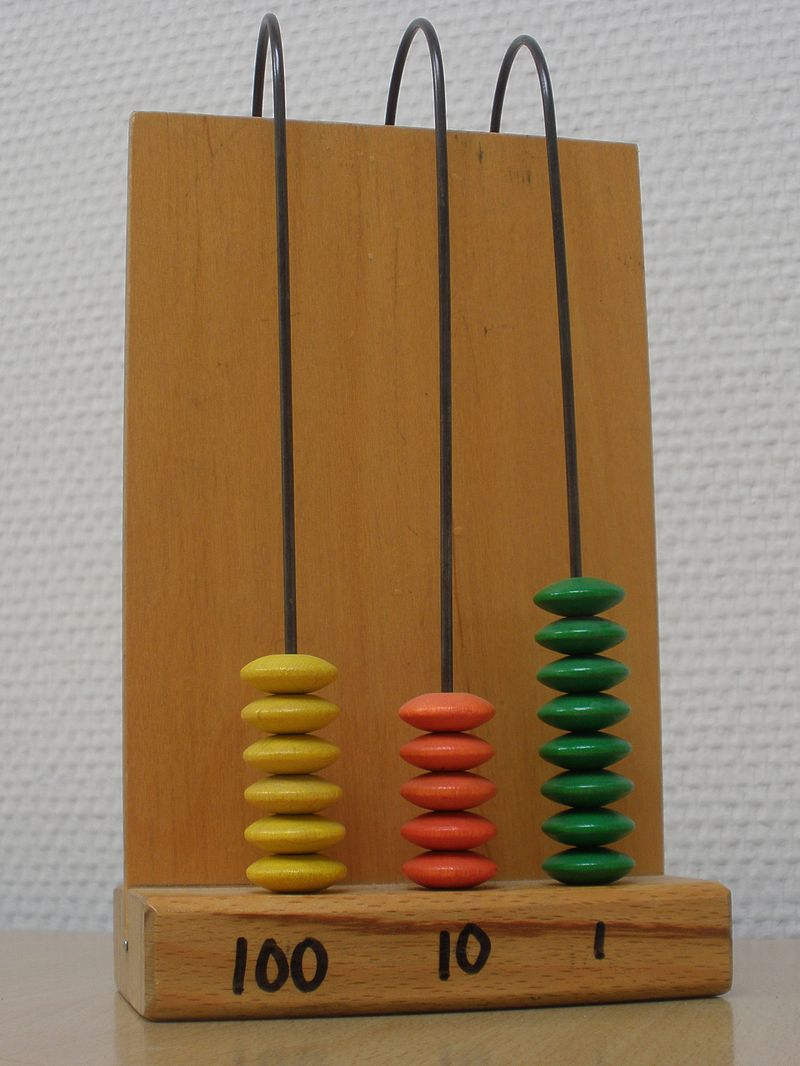
\includegraphics[width=0.6\textwidth]{Pictures/Abacus_school.JPG}\\
Een Abacus waarop het getal 658 is gezet.\\{\tiny(Bron: Wikipedia)}\\
\end{center}
\end{minipage}
\end{exercise}

\begin{exercise}[Up and Down]\mbox{}\\
Maak een copy van de package van de opdracht Abacus en gebruik dit als basis voor de opdrachten A en B. 
\subsubsection{A:} 
Pas de publisher aan zodat hij nu willekeurig het woord “plus”, “min” of “keer” stuurt samen met het willekeurige getal. Voorbeeld van berichten op de topic:


\begin{minipage}{0.9\linewidth}
\begin{lstlisting}[style=DOS, firstnumber=0]
plus 8 
min 9 
plus 3 
plus 0 
plus 2 
keer 3
\end{lstlisting}
\end{minipage}

\subsubsection{B:}
Pas ook de subscriber aan, zodat hij de nieuwe berichten van de publisher kan verwerken. Ontvangt de subscriber een bericht met het woord “plus” dan verwerkt hij het getal met een plus. Ontvangt de subscriber een bericht het woord “min” verwerkt hij het getal met een min. Ontvangt de subscriber een bericht het woord “keer” verwerkt hij het getal met een keer. Als het eerste cijfer met het woord “keer” komt, dan verwerkt hij dat als 0 * <getal>.
\end{exercise}

\newpage %!!!!!newpage!!!!!!!

\begin{exercise}[Libellebil]\mbox{}\\
Bekijk onder staande code en beantwoord de onderstaande vragen zonder de code uit te voeren.

\begin{enumerate}
    \item Wat is de service die serviceNode verleend?
    %het draait de string om%
    \item Maak het .srv bestand dat wordt gebruikt door serviceNode.
    %zie codevoorbeelden%
\end{enumerate}

\begin{minipage}{0.9\linewidth}
\begin{lstlisting}[language=C++, firstnumber=0]
#include "rclcpp/rclcpp.hpp"
#include "ServiceNode.h"

using std::placeholders::_1;
using std::placeholders::_2;

ServiceNode::ServiceNode(): Node("ServiceNode"){
    service_ = this->create_service<srvcli_libellebil::srv::Word>(
            "words", 
            std::bind(&ServiceNode::handleService, this, _1, _2)
    );
}

std::string ServiceNode::esrever(std::string word){
    for(size_t i=0; i<word.size()/2; i++){    
        std::swap(word[i], word[word.size()-i-1]);
    }
    return word;
}

void ServiceNode::handleService( 
    const std::shared_ptr<srvcli_libellebil::srv::Word::Request> request,
    std::shared_ptr<srvcli_libellebil::srv::Word::Response> response
){
  std::string outputWord = esrever(request->input_word);

  bool isIt = outputWord == request->input_word;

  response->output_word = outputWord;
  response->is_it = isIt;
}
\end{lstlisting}
\end{minipage}


\end{exercise}

\begin{exercise}[Wijzerplaat]\mbox{}
\begin{minipage}{0.5\textwidth}
\begin{enumerate}
    \item Maak een ROS2 node die functioneert als een analoge klok. De node publiceert de huidige stand van de wijzers eens per seconde.
    \item Maak van de analoge klok node ook een service server. Door middel van de service kan men de klok stopzetten en weer starten.
\end{enumerate}.
\end{minipage}\hfill 
\begin{minipage}{0.4\textwidth}
\begin{center}
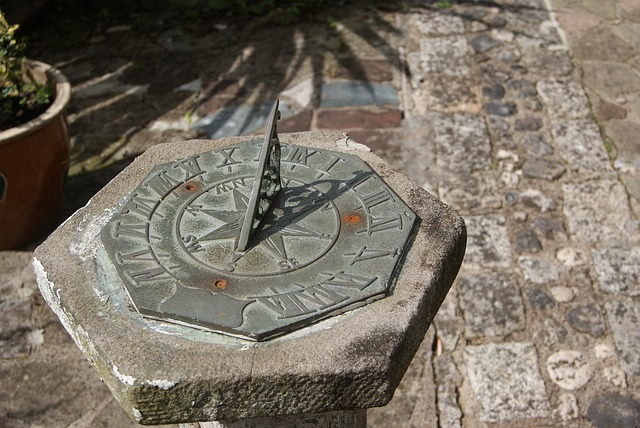
\includegraphics[width=0.95\textwidth]{Pictures/cc_pixabay_zonnwijzer.jpg}\\
Een zonnewijzer.\\
{\tiny(Afbeelding van Mark Caldicott via \url{pixabay.com})}
\end{center}
\end{minipage}
\end{exercise}

\newpage %!!!!!!!!!!!!!!!!newpage!!!!!!!!!

\begin{exercise}[Actie]\mbox{}%Lukt mij niet op een (leuke) zinnige leesopdracht te maken. Daarom maar toevlucht gezocht naar theorievragen. Een suggesties voor een code-leesopdracht over een action-node is welkom.
\begin{enumerate}
    \item Welke berichten bij een action server/client moet je zelf definiëren in de Action message structure?
    \item Welke berichten zijn al voorgedefinieerd bij een action server/client?
\end{enumerate}
\end{exercise}

\begin{exercise}[Conway’s action]\mbox{}\\
Schrijf een ROS action server die de rij van Conway kan bepalen. De rij van Conway staat ook wel bekend als de Look-and-say sequence, omdat het volgende element in de rij wordt gevormd door het huidige element te beschrijven. Meer informatie over de Look-and-say-sequence kan men vinden op:
\begin{itemize}
    \item \url{https://nl.wikipedia.org/wiki/Rij_van_Conway}
    \item \url{https://www.youtube.com/watch?v=ea7lJkEhytA}
\end{itemize}

De action server krijgt als goal de integers \textit{x} en \textit{n} mee. Aan de hand hiervan moet de node de rij van Conway bepalen die begint met \textit{x} en die \textit{n} lang is. De action server geeft elk tussenresultaat terug als feedback naar de action client. Voorbeelden van input van de service en de output staan in de tabel hieronder. Je mag aannemen dat \textit{x} en \textit{n} altijd positief zijn.

\vspace{0.5cm}

\begin{minipage}{0.6\textwidth}

\begin{tabular}{|l|l|p{6cm}|} \hline
\textbf{x} & \textbf{n} & \textbf{Output}  \\ \hline
5 & 3 & 15, 1115, 3115 \\ \hline
367 & 5 & 131617, 111311161117, 311331163117, 1321232116132117, 1113121112131221161113122117  \\ \hline
1 & 7 & 11, 21, 1211, 111221, 312211, 13112221, 1113213211 \\ \hline
9 & 4 & 19 , 1119, 3119, 132119 \\ \hline
\end{tabular}

\end{minipage}\hfill 
\begin{minipage}{0.3\textwidth}
\begin{center}
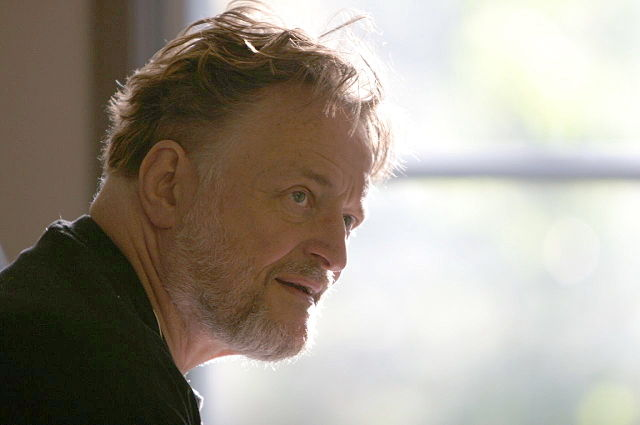
\includegraphics[width=\textwidth]{Pictures/640px-John_H_Conway_2005.jpg}\\
De wiskundige John Conway (1937 - 2020).\\{\tiny(Bron: Wikipedia)}\\
\end{center}
\end{minipage}


\vspace{1cm}
\noindent Schrijf ook een action client te testen ook een service client en zorg dat de package voldoet aan de ROS2 conventies. \\

% lukt het de student niet om de het algoritme van conways service te implementeren. Geef deze dan of laat de student een andere service maken. Leerdoel is om een ros2 service te maken.
\end{exercise}

\begin{exercise}[Pijpleiding]\mbox{}\\
Koppel de nodes gemaakt in opdracht 7.5, 7.7 en 7.9 aan elkaar. Bedenk zelf welke nodes met elkaar communiceren. Het kan zijn dat de eerder geschreven nodes een extra of andere communicatierol krijgen en je dus zaken aan je code moet toevoegen.
\end{exercise} 

% Appendices
\begin{appendices}
\renewcommand{\chaptername}{Appendix} % fix header
\renewcommand{\appendixname}{} % remove 'Appendix' from chapter name in toc
\chapterimage{cc_pixabay_header_lego_builders}
\addappheadtotoc % Add a section header 'Appendices' to toc
%add below the appendixes:
\chapter{HelloNode package}
\label{chp:HelloNode_package}
In hoofdstuk \ref{chp:ROS_nodes} hebben we gekeken naar hoe de C++code voor een simpele ROS 2 node er uitziet. In dit hoofdstuk maken we van HelloNode van codevoorbeeld \ref{code:hello_world_ROSnode_hpp}, \ref{code:hello_world_ROSnode_cpp} en \ref{code:hello_world_ROSnode_main} een werkende package\footnote{De code is ook te vinden op de git van deze reader.}. Dit hoofdstuk is geen vervanging de tutorials op \url{https://index.ros.org/doc/ros2/Tutorials/}, maar geeft de lezer wel een inzicht en toelichting in welke stappen doorlopen moeten worden voor het maken van een ROS 2 Foxy Fitzroy package op een Linux-machine. Een package is een collectie van één of meerdere ROS-nodes die logische wijs bij elkaar horen. Een typisch ROS-project bestaat uit meerdere packages.

Mocht je ROS 2 nog niet hebben geïnstalleerd dan kan dat via. In deze uitleg gaan we uit van ROS 2 versie \textit{Foxy Fitzroy}.
\begin{center}
    \url{https://docs.ros.org/en/foxy/Installation.html}
\end{center}

\subsubsection{ROS 2 environment}
Als we met ROS aan de slag gaan moeten we altijd eerst de ROS 2 environment starten:
\begin{lstlisting}[style=DOS, caption={}, firstnumber=0, label={}]
 source /opt/ros/foxy/setup.bash
\end{lstlisting}

\subsubsection{Workspace}
Je kan de packages in een bestaande workspace plaatsen. Als je nog geen workspace\footnote{Een workspace is een bestand of folder dat de gebruiker de mogelijkheid geeft om allerlei source code bestanden en resources te verzamelen en mee te werken als \'e\'en samenhangend geheel (vrij vertaald van wikipedia). Dit betekent dat als je een workspace hebt ongerelateerde bestanden (bijvoorbeeld zowel bestanden uit deze reader als andere projecten) dat je een rommel aan het maken bent.} hebt of het netjes in een nieuwe workspace wil plaatsen, dan moet je eerst een folder aanmaken. Wij noemen onze folder \textit{reader\_ws}. In deze workspace plaatsen we alle packages die in deze reader worden behandeld. Het is een ROS-conventie om de packages in de \textit{src} (source) folder van de workspace te plaatsen. We maken onze workspace met src-folder met de volgende commandline:
\begin{lstlisting}[style=DOS, caption={}, firstnumber=0, label={}]
 mkdir -p ~/reader_ws/src
\end{lstlisting}

\subsubsection{Het maken van een lege package}
We bewegen onszelf naar de folder waar we de packages gaan plaatsen:
\begin{lstlisting}[style=DOS, caption={}, firstnumber=0, label={}]
 cd ~/reader_ws/src
\end{lstlisting}
Het maken van een package gaat met de commando \textit{ros2 pkg create --build-type ament\_cmake <package\_name>}\footnote{Dit commando komt met nog veel meer functionaliteit. Bijvoorbeeld kunnen de dependencies automatisch aan \textit{package.xml} en \textit{CMakeLists.txt} toegevoegd worden door gebruik te maken van de flag \textit{--dependencies}.}. Het commando maakt voor ons de folderstructuur van de package en de bestanden \textit{CMakeLists.txt} en \textit{package.xml}. Deze bestanden helpen ons met het bouwen van de package en het starten van verschillende packages. We noemen onze package Hello:
\begin{lstlisting}[style=DOS, caption={}, firstnumber=0, label={}]
ros2 pkg create --build-type ament_cmake hello
\end{lstlisting}

\subsubsection{Code in de package}
Gebruik je favouriete tekst-editor om \textit{HelloNode.cpp} te maken zoals beschreven in codevoorbeelden \ref{code:hello_world_ROSnode_hpp}, \ref{code:hello_world_ROSnode_cpp} en \ref{code:hello_world_ROSnode_main}. Plaats HelloNode.cpp en main.cpp in de folder \textit{~/reader\_ws/src/Hello/src} en HelloNode.hpp in de folder \textit{~/reader\_ws/src/Hello/include/hello}. De inhoud van onze folder is nu:
\begin{lstlisting}[caption={De folder structuur inclusief bestanden van de package Hello.}, firstnumber=0, label={}]
\reader_ws
    \src
        \hello
            CMakeLists.txt
            package.xml
            \include
                \hello
                    HelloNode.hpp
            \src
                HelloNode.cpp
                main.cpp
\end{lstlisting}

\subsubsection{Package.xml}
In package.xml geven we informatie over de package Hello zoals de naam, beschrijving, license en de dependencies. Deze informatie is niet alleen handig voor anderen die de package gaan gebruiken, maar de dependencies zijn noodzakelijk voor het correct werken met ROS 2. Open package.xml in je favoriete teksteditor en zorg dat het de onderstaande inhoud heeft. Let vooral op regel 11. Hiermee zeggen we dat onze package afhankelijk is van \textit{rclcpp}.

\begin{lstlisting}[style=XML, firstnumber=0]
<?xml version="1.0"?>
<?xml-model href="http://download.ros.org/schema/package_format3.xsd" schematypens="http://www.w3.org/2001/XMLSchema"?>
<package format="3">
  <name>hello</name>
  <version>0.0.0</version>
  <description>A node that says hello to the world!</description>
  <maintainer email="Jorn.Bunk@han.nl">Jorn Bunk</maintainer>
  <license>Attribution 4.0 International (CC BY 4.0)</license>

  <buildtool_depend>ament_cmake</buildtool_depend>

  <depend>rclcpp</depend>

  <test_depend>ament_lint_auto</test_depend>
  <test_depend>ament_lint_common</test_depend>

  <export>
    <build_type>ament_cmake</build_type>
  </export>
</package>
\end{lstlisting}
\subsubsection{CMakeLists.txt}
In de CMakeLists.txt geven we de build instellingen van onze package. Open CMakeLists.txt in je favoriete teksteditor en zorg dat het de onderstaande inhoud heeft. De standaard CMakeLists.txt bevat ook een aantal onderdelen die we niet nodig hebben\footnote{De standaard CMakeLists.txt bevat ook een aantal zaken niet die bij sommige packages wel nodig zijn, bijvoorbeeld als de package ook messages definieert.}, deze opgeruimd. Er 3 belangrijke onderdelen aan dit bestand. Allereerst hebben we de \textit{find\_package()}-functies waarin de dependencies moeten worden genoemd. In het geval van deze package is dat enkel \textit{rclcpp} en \textit{ament\_cmake}. Die laatste is standaard. Het tweede onderdeel is het toevoegen van de executable met \textit{add\_exutable()} en \textit{ament\_target\_dependencies()}, zodat ROS 2 de package kan uitvoeren. We moeten hierbij onze executable een naam geven. Er is hier voor de naam \textit{greeter} gekozen. Als laatste moeten we ook zorgen dat ROS 2 onze executable kan vinden. Dit doen we met de functie \textit{install()}. Een package kan ook bestaan uit meerdere executables. Hiervoor moeten regel 18 en 19 worden herhaald met de instellingen van de andere executables en moeten de namen van de executables worden toegevoegd aan het lijstje met TARGETS (regel 22/23).

\begin{lstlisting}
cmake_minimum_required(VERSION 3.5)
project(hello)

# Default to C++14
if(NOT CMAKE_CXX_STANDARD)
  set(CMAKE_CXX_STANDARD 14)
endif()

if(CMAKE_COMPILER_IS_GNUCXX OR CMAKE_CXX_COMPILER_ID MATCHES "Clang")
  add_compile_options(-Wall -Wextra -Wpedantic)
endif()

# find dependencies
find_package(ament_cmake REQUIRED)
find_package(rclcpp REQUIRED)

# The path to our header files:
# make sure the folder inside /include had the same name as the project!
include_directories(include/${PROJECT_NAME}/)

# add the executable
add_executable(greeter src/main.cpp src/HelloNode.cpp)
ament_target_dependencies(greeter rclcpp)

# Making ROS 2 able to find our package:
install(TARGETS
  greeter
  DESTINATION lib/${PROJECT_NAME})

ament_package()
\end{lstlisting}

\subsubsection[Bouwen en rennen]{Bouwen en rennen\footnote{Dit is een grapje.}}
Waarschijnlijk heb je al de dependencies die nodig zijn voor de package Hello, desondanks is het een goede gewoonte om te controlleren op missende dependencies. Dit doe je door dit in de hoofdfolder van je workspace (\textit{reader\_ws}) het volgende te runnen:

\begin{lstlisting}[style=DOS, caption={}, firstnumber=0, label={}]
 rosdep install -i --from-path src --rosdistro foxy -y
\end{lstlisting}

\noindent Het bouwen van de package doen we, nog steeds vanuit de folder \textit{reader\_ws}, nu met: 
\begin{lstlisting}[style=DOS, caption={}, firstnumber=0, label={}]
 colcon build --packages-select hello
\end{lstlisting}

\noindent De package is nu gebouwd. Om onze package te runnen moeten we eerst de setup files uitvoeren:
\begin{lstlisting}[style=DOS, caption={}, firstnumber=0, label={}]
 . install/setup.bash
\end{lstlisting}

\noindent De node kunnen we nu starten met:
\begin{lstlisting}[style=DOS, caption={}, firstnumber=0, label={}]
ros2 run hello greeter
\end{lstlisting}

\noindent Gebruik CTRL+C om de node te stoppen. 
\chapterimage{cc_pixabay_header_doors}
\chapter{Frequently Asked Questions}

\section{ROS?!}

\subsection{ondanks dat ik een package bouw blijft hij de oude gecompileerde bestanden uitvoeren?}
Waarschijnlijk bouw en run je op twee verschillende plekken. Waarschijnlijk ben je aan het bouwen in de package in plaats van in de hoofdfolder van je workspace.

\subsection{Ik heb al heel veel geprobeerd, maar de fout blijft maar bestaan?}
Waarschijnlijk bouw en run je op twee verschillende plekken. Waarschijnlijk ben je aan het bouwen in de package in plaats van in de hoofdfolder van je workspace.



\subsection{Rare errors}
\textit{Ik krijg rare errors?}

Waarschijnlijk ben je vergeten de ROS 2 environment te activeren door middel van:
\begin{lstlisting}[style=DOS, caption=Hello world, firstnumber=0, label={code:DOS_voorbeeld}]
 source /opt/ros/foxy/setup.bash
\end{lstlisting}
Dit moet je doen in elke terminal voordat je iets met ROS 2 doet (zowel runnen van nodes als het bouwen van packages).

\subsection{Colcon build geeft warning}
\textit{WARNING:colcon.colcon\_ros.prefix\_path.ament:The path '/een/path/' in the environment variable AMENT\_PREFIX\_PATH doesn't exist}
Waarschijnlijk heb je een package een andere naam gegeven. Deze warning kan geen kwaad. Wil je van de warning af? Verwijder dan de folders \textit{install}, \textit{build} en \textit{log} (rm -r build log install) en start een nieuwe terminal\footnote{Dit kan waarschijnlijk ook door AMENT\_PREFIX\_PATH te resetten. Laat even weten als je het command hiervoor hebt.}.

\subsection{Colcon build geeft error  message/service/action van andere package}
\begin{enumerate}
\item \textit{CMake Error at CMakeLists.txt:24 (find\_package):
  By not providing "Findpackage\_name" in CMAKE\_MODULE\_PATH this
  project has asked CMake to find a package configuration file provided by
  "packagename", but CMake did not find one.}

Je bent vergeten in je package.xml de package met de message/service/action toe te voegen aan aan het rijtje met <depend> </depend>.

\item \textit{CMake Error at /opt/ros/foxy/share/amen\_cmake\_target\_dependencies/cmake/ament\_target\_dependencies.cmake:77 (message):
  ament\_target\_dependencies() the passed package name `package\_name'}

Je bent vergeten de package met de message/action/service toe te voegen als dependencie aan je CMakeLists.txt

\end{enumerate}
\subsection{Message/service/action met een string}
\textit{Een string die ik via een message/service/action heb verstuurd print als rare tekens?}

Waarschijnlijk ben je vergeten om de functie \textit{c\_str()} te gebruiken. Je drukt nu de pointer af. Voorbeeld: Als je string in \textit{data} zit, dan krijg je de string met \textit{data.c\_str()}.

\subsection{Custom message/service/action hpp includeren}
\textit{Als ik een custom message/service/action heb gemaakt hoe heet dan de hpp die ik moet includeren?}
Een custom message/service/action wordt door ROS omgezet naar een .hpp die je moet includeren in de C++ bestanden die gebruik maken van de message/service/action. Het door ROS gemaakte .hpp-bestand hanteert een andere bestandsnaamconventie.
De naam van een custom message/service/action moet beginnen met een hoofdletter. Het hpp-bestand dat je moet includeren heeft vervolgens geen hoofdletters, maar voor elke hoofdletter, met uitzondering van de eerste, wordt een underscore (\_) geplaatst. Het pad van het hpp-bestand is gelijk aan dat van je custom message/action/service. In de codevoorbeelden die komen bij deze reader op de git-omgeving kan je hier voorbeelden van vinden.

\subsection{Error rond $>$ en ::SharedPointer bij het maken van een action Node}
Waarschijnlijk ben je rclcpp\_action vergeten toe te voegen aan je package.xml.

\subsection{Vtable}
\textit{undefined reference to `vtable for \dots'.}
Waarschijnlijk heeft je class/node nog geen destructor.

\section{Arduino?!}

\subsection{Serial Communicatie traag }
\textit{Als ik communiceer met serial op arduino kost dat veel tijd.}

Haal niet steeds het bericht op uit de buffer. Kijk eerst of er iets in de buffer staat door gebruik te maken van de functie \textit{Serial.available()}: \url{https://www.arduino.cc/reference/en/language/functions/communication/serial/available/}



\end{appendices}
%----------------------------------------------------------------------------------------
%	References
%----------------------------------------------------------------------------------------

% below is needed if we want to add a bibliography

%\chapterimage{header-proof.png} % Table of contents heading image

%\pagestyle{empty} % No headers

%\printbibliography\addcontentsline{toc}{chapter}{Bibliografie} 

%\cleardoublepage % Forces the first chapter to start on an odd page so it's on the right

%\pagestyle{fancy} % Print headers again

\end{document}
